\documentclass[12pt]{book}
\usepackage[utf8]{inputenc}
\usepackage[T1]{fontenc}
\usepackage{mathptmx}
\usepackage{geometry}
\usepackage{mathtools}
\usepackage[english]{babel}
\usepackage{graphicx}
\usepackage{subcaption}
\usepackage{stackengine}
\usepackage[os=win]{menukeys}
\usepackage{hyperref}
\usepackage{minted}
\usepackage{xcolor}
\usepackage{tikz}
\usepackage[yyyymmdd,hhmmss]{datetime}
\usepackage{etoolbox}
\usepackage[inline]{enumitem}
\usepackage{pdfpages}

\newcommand{\WindowsLogo}{\raisebox{-0.1em}{
\includegraphics[height=0.8em]{images/logo/Windows_3_logo_simplified}}}
%\newcommand{\PowerLogo}{\raisebox{-0.1em}{
\includegraphics[height=0.8em]{images/logo/power}}}
\newcommand{\WinKey}{\keys{\WindowsLogo}}
\newcommand{\PowerKey}{\keys{\PowerLogo}}

\patchcmd{\thebibliography}{\section*{\refname}}{}{}{}

\addto\captionsenglish{\renewcommand{\contentsname}{Daftar Isi}}
\addto\captionsenglish{\renewcommand{\figurename}{Gambar}}

\hypersetup{
	colorlinks=true, %set true if you want colored links
	linktoc=all,     %set to all if you want both sections and subsections linked
	linkcolor=blue,  %choose some color if you want links to stand out
	urlcolor=blue,   %url color
}

\geometry{
	a4paper,
	left=10mm,
	right=10mm,
	top=15mm,
	bottom=15mm,
}

\date{}

\hypersetup{citecolor=black}

\definecolor{LightGray}{gray}{0.95}

%\pagecolor[rgb]{0.1,0.1,0.1}
%\color[rgb]{1,1,1}

\begin{document}

	\frontmatter
	\begin{titlepage}
		\centering
		{\LARGE \bf Pengenalan MATLAB dan Dasar Pemrogramannya}
		\vfill
		{\Large Achmadi ST MT}
		\vfill
		
\includegraphics[width=250pt]{images/logo/logoviblab}
		\vfill
		\vfill
		\noindent This book written:\\
		Update: {\today} at \currenttime\\
	\end{titlepage}

	%%%%%%%%%%%%%%%%%%%%%%%%%%%%%%%%%%%%%%%%%%%%%%%%%%%%%%%%%%%%%%%%%

	\newpage
	\tableofcontents

	%%%%%%%%%%%%%%%%%%%%%%%%%%%%%%%%%%%%%%%%%%%%%%%%%%%%%%%%%%%%%%%%%

	\newpage
	\chapter{Disclaimer}

	MATLAB adalah merek dagang dari The MathWorks, Inc.
	The MathWorks sendiri tidak menjamin akurasi isi buku ini.
	Penggunaan buku dalam kaitan perangkat lunak MATLAB tidak bermaksud promosi atau sponsor dari MathWorks.
	\\
	\\
	Konten buku ini disarikan dari buku \textit{"Chemical Engineering Computation with MATLAB"} oleh Yeong Koo Yeo,
	dipublikasikan oleh CRC Press tahun 2001.

	%%%%%%%%%%%%%%%%%%%%%%%%%%%%%%%%%%%%%%%%%%%%%%%%%%%%%%%%%%%%%%%%%

	\newpage
	\chapter{Penggunaan Buku}

	\section{Umum}
	Buku ini dibuat dengan tujuan penggunaan utama sebagai panduan digital untuk mempermudah search dan copy-paste.
	Anda tidak perlu mencetak buku ini ke bentuk kertas.
	Seluruh navigasi buku ini diharapkan menggunakan klik ke hyperlink di Daftar Isi,
	atau menggunakan tampilan \textbf{Index} yang tersedia di \textbf{SideBar} program pembaca PDF yang anda gunakan.

	\section{Petunjuk}
	Beberapa petunjuk yang digunakan di buku ini:
	\begin{itemize}
		\item \textbf{Cetak Tebal}: Menginformasikan identifier (keyword, variabel, fungsi, alamat, nama file, dst) yang berada di suatu paragraf
		\item \textit{Cetak Miring}: Bersama simbol panah (->) dan simbol lain, menginformasikan langkah-langkah klik menu/tombol.
		\item \textbf{TIPS:} Menginformasikan hal-hal yang dapat membantu atau pengetahuan tambahan.
		\item \textbf{PERINGATAN:} Menginformasikan hal-hal yang bener-benar harus diperhatikan.
	\end{itemize}

	\section{Penulisan Kode}
	Untuk penulisan kode, akan digunakan tiga bentuk:
	\begin{enumerate}
		\item IN dan OUT. Berupa bagian kode, dengan:
		\begin{itemize}
			\item Baris dengan tanda \textbf{Prompt} (>>) adalah Input.
			Anda tidak perlu ketik ulang prompt.
			\item Baris dibawahnya tanpa ada tanda \textbf{Prompt} (>>) adalah contoh Output
		\end{itemize}

		\begin{minted}[frame=lines,framesep=2mm,fontsize=\small,bgcolor=LightGray]{matlab}
>> input
output
		\end{minted}

		\item IN saja. Hanya sebagai input dengan ditandai \textbf{Prompt} (>>).
		Anda tidak perlu ketik ulang prompt.
		Contoh Output disini tidak ditampilkan.

		\begin{minted}[frame=lines,framesep=2mm,fontsize=\small,bgcolor=LightGray]{matlab}
>> input
		\end{minted}

		\newpage
		\item Script/Function. Kode ditulis sebagai file script atau function tanpa ada tanda \textbf{Prompt} (>>) sama sekali.

		\begin{minted}[frame=lines,framesep=2mm,fontsize=\small,bgcolor=LightGray]{matlab}
function y=tambah(a,b)
	y = a + b
end
		\end{minted}
	\end{enumerate}

	\section{Prinsip Belajar}

	Matematika dan Pemrograman (termasuk MATLAB) adalah sebuah bahasa.
	Mempelajari suatu bahasa baru memang selalu berat dan menguras pikiran.
	\\
	\\
	Cara terbaik mempelajari suatu bahasa adalah memahami konsep-inti, tidak menghafal,
	dan menggunakannya sesering mungkin.
	\\
	\\
	Jangan takut dengan panjangnya suatu kode/persamaan,
	karena semua itu dibangun dari unit-unit sederhana.

	%%%%%%%%%%%%%%%%%%%%%%%%%%%%%%%%%%%%%%%%%%%%%%%%%%%%%%%%%%%%%%%%%

	\newpage
	\mainmatter
	\chapter{Program MATLAB}

	Program MATLAB adalah program komputasi yang digunakan secara universal dalam bidang Sains dan Engineering.
	Secara garis besar, MATLAB adalah program kalkulator super canggih yang dapat menyelesaikan proses perhitungan kompleks.

	\section{Memulai Program}

	Anda dapat memulai program MATLAB sebagaimana program lainnya.

	\subsection{Windows}
	Untuk Windows 7, 8 , dan 10, Tekan tombol \textit{Start Windows} (\keys{\WindowsLogo}) dan ketik "MATLAB" untuk mencari program MATLAB yang terinstal.
	Tekan \textit{Enter} (\keys{\return}) untuk memulai
	\begin{figure}[!ht]
		\centering
		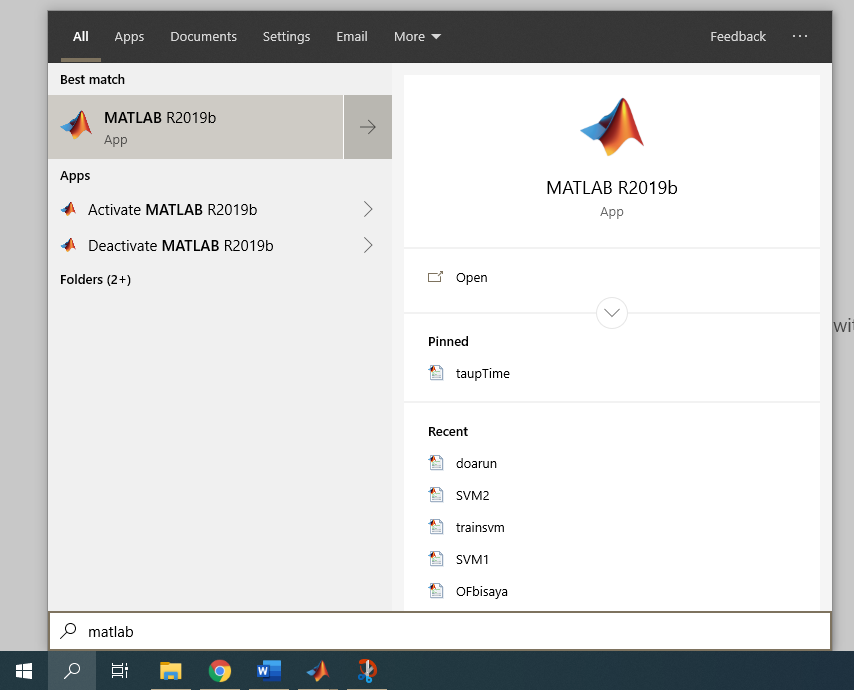
\includegraphics[width=250pt]{images/startmenuwin}
		\caption{Start MATLAB Windows}
	\end{figure}

	\subsection{GNU/Linux}
	Untuk GNU/Linux seperti ArchLinux, Manjaro, atau Ubuntu, tekan \textit{Start Menu} -> MATLAB.
	\begin{figure}[!ht]
		\centering
		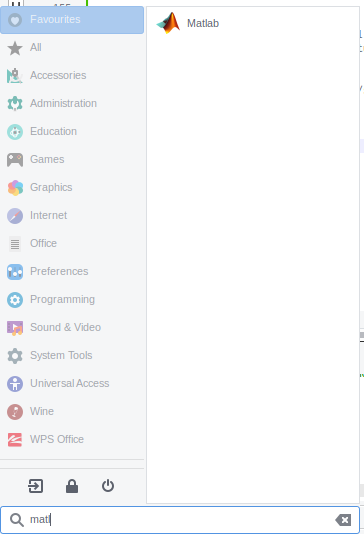
\includegraphics[width=200pt]{images/startmenumate}
		\caption{Start MATLAB GNU/Linux}
	\end{figure}

	\newpage
	Metode lainnya adalah memanggil program matlab dengan Terminal/Bash Emulator dan masukkan perintah:
	\begin{minted}[frame=lines,framesep=2mm,fontsize=\small,bgcolor=LightGray]{bash}
$> matlab
	\end{minted}

	\subsection{MacOS}

	Menyusul

	\newpage
	\section{Bagian Antar Muka}

	Antar Muka (Interface) program MATLAB dapat berbeda antara satu pengguna dan pengguna lainnya.
	Berikut salah satu tampilan default yang umum dipakai:

	\begin{figure}[!ht]
		\centering
		\begin{subfigure}[b]{0.75\textwidth}
			\includegraphics[width=\textwidth]{images/matlabiface}
		\end{subfigure}
		\begin{subfigure}[b]{0.2\textwidth}
			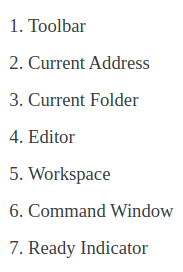
\includegraphics[width=\textwidth]{images/matlabpart}
		\end{subfigure}
		\caption{Bagian Antar Muka}
	\end{figure}

	\subsection{Default Layout}

	Jika ingin untuk mengembalikan penataan (Layout) antar muka program, anda dapat melakukannya melalui Toolbar.
	Pilih tab \textit{Home} -> \textit{Layout}, kemudian pilih \textit{Default} atau \textit{Two-Column}.

	\begin{figure}[!ht]
		\centering
		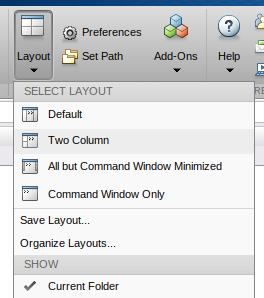
\includegraphics[width=150pt]{images/matlablayout}
		\caption{Penataan MATLAB}
	\end{figure}

	\subsection{Toolbar}
	Toolbar disini bertindak sama seperti Toolbar pada Microsoft Office.
	Disini tersedia beragam perintah dalam bentuk icon yang dapat diklik.

	\newpage
	Tab yang tersedia antara lain:
	\begin{itemize}
		\item \textit{Home}. Berisi perintah dasar untuk mengolah file, variable, pengaturan program, dan layout.
		\item \textit{Plot}. Berisi perintah pengolahan plot langsung dari variable yang tersedia di Workspace.
		\item \textit{Apps}. Berisi perintah tambahan dari toolbox atau addon yang terinstal.
		\item \textit{Editor}. Berisi perintah untuk mengolah file, mengelola jalannya suatu skrip, dan perintah editing.
		Hanya muncul jika Editor diaktifkan.
		\item \textit{Publish}. Berisi perintah untuk membantu publikasi dan berbagi kode sumber melalui website MATLAB.
		Hanya muncul jika Editor diaktifkan.
		\item \textit{View}. Berisi perintah untuk mengolah tampilan kode sumber yang sedang diedit.
		Hanya muncul jika Editor diaktifkan.
	\end{itemize}

	\subsection{Current Address}

	Current Address digunakan untuk menunjukkan alamat folder yang sedang aktif dan membantu navigasi berpindah folder.
	Icon tersedia antara lain panah navigasi (seperti pada webbrowser), icon folder untuk jelajah folder dengan program \textit{file-manager},
	teks alamat folder yang dapat diedit, icon panah bawah untuk history, dan icon lup untuk mencari.

	Untuk berpindah folder, anda dapat input teks alamat folder secara manual.
	Anda cukup klik alamat dan saat muncul cursor, anda dapat edit/paste alamat dan kemudian tekan Enter (\keys{\return}) untuk berpindah folder.

	\begin{figure}[!ht]
		\centering
		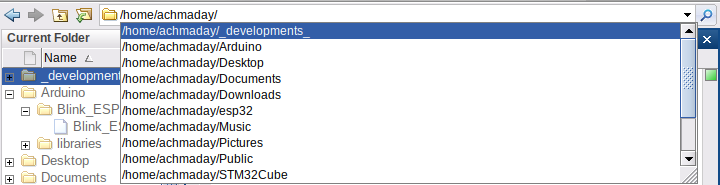
\includegraphics[width=350pt]{images/addressbaredit}
		\caption{Pindah Alamat}
	\end{figure}

	\textbf{TIPS:} Alamat di atas adalah format alamat untuk Unix (Linux/MacOS).
	Untuk Windows, alamat akan memiliki format dimulai "\textbf{C:\textbackslash}" atau "\textbf{D:\textbackslash}" sesuai drive.\\

	Selain itu, anda juga dapat menggunakan history untuk berpindah folder.
	Tekan icon panah bawah di sisi kanan alamat.

	\begin{figure}[!ht]
		\centering
		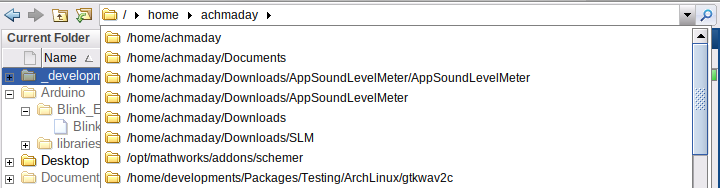
\includegraphics[width=350pt]{images/addressbarhistory}
		\caption{History Alamat}
	\end{figure}

	\newpage
	\subsection{Current Folder}

	Current Folder menampilkan file dan folder di alamat yang sedang aktif.
	Anda dapat membuka, menghapus, membuat, dan memindahkan file disini.
	Anda juga dapat berpindah folder dengan double-klik folder yang tersedia.

	\begin{figure}[!ht]
		\centering
		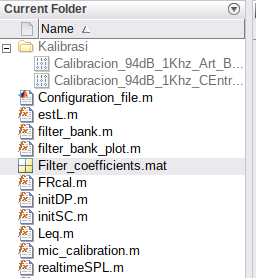
\includegraphics[width=150pt]{images/currentfolder}
		\caption{Current Folder}
	\end{figure}

	\subsection{Command Window}

	Command Window adalah bagian utama MATLAB dimana anda memasukkan perintah-perintah teks untuk diproses oleh MATLAB.
	Hasil proses juga akan ditampilkan disini.

	\begin{figure}[!ht]
		\centering
		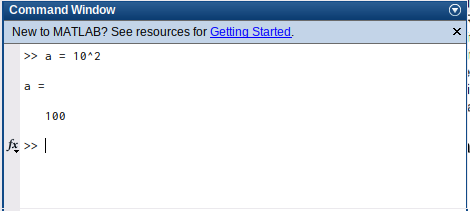
\includegraphics[width=250pt]{images/commandwindow}
		\caption{Command Window}
	\end{figure}

	sebagai percobaan, coba masukkan perintah berikut dan tekan ENTER (\keys{\return})

	\begin{minted}[frame=lines,framesep=2mm,fontsize=\small,bgcolor=LightGray]{matlab}
>> a = 10^2
a =
   100
	\end{minted}

	\subsubsection{TIPS:}

	Berikut beberapa tips yang sangat membantu:

	\begin{itemize}
		\item \textbf{Tanda Prompt}

		Prompt digunakan sebagai penanda baris dimana anda dapat memasukkan perintah ke MATLAB.
		Tanda prompt berupa dua panah ke kanan (\textbf{>>}) di Command Window.

		\item \textbf{Menghentikan Proses}

		Apabila terjadi ingin menghentikan suatu proses eksekusi perintah,
		anda dapat menggunakan kombinasi tombol CTRL+c (menekan tombol \keys{Ctrl} dan huruf \keys{c} bersamaan di keyboard).

		Sebagai contoh, masukkan perintah berikut:
		\begin{minted}[frame=lines,framesep=2mm,fontsize=\small,bgcolor=LightGray]{matlab}
>> while(true);pause(1);end
		\end{minted}

		Disini terlihat ada jarak satu baris namun tidak ada tanda Prompt,
		menandakan MATLAB sedang sibuk dan tidak dapat menerima perintah lebih lanjut.

		Untuk menghentikan proses, tekan \keys{Ctrl} dan huruf \keys{c} bersamaan.

		\item \textbf{Semi-Colon}

		Tanda Semi-Colon (;), memiliki 2 fungsi:
		\begin{enumerate}
			\item Sebagai pemisah statement untuk satu baris.
			Sebagai contoh berikut deklarasikan 3 variable.
			\begin{minted}[frame=lines,framesep=2mm,fontsize=\small,bgcolor=LightGray]{matlab}
>> varA = 10
>> varB = 20
>> varC = 30
			\end{minted}

			Anda juga dapat menuliskannya sebagai:
			\begin{minted}[frame=lines,framesep=2mm,fontsize=\small,bgcolor=LightGray]{matlab}
>> varA = 10; varB = 20; varC = 30
			\end{minted}

			\item Untuk menyembunyikan (suppress) respon output untuk perintah yang dijalankan
			Sebagai contoh perintah berikut:
			\begin{minted}[frame=lines,framesep=2mm,fontsize=\small,bgcolor=LightGray]{matlab}
>> varA = 10
varA =
	10
			\end{minted}

			Terlihat bahwa MATLAB akan merespon memberitahukan bahwa varA bernilai 10.
			Jika perintah di atas diakhiri tanda semi-colon (;):

			\begin{minted}[frame=lines,framesep=2mm,fontsize=\small,bgcolor=LightGray]{matlab}
>> varA = 10;
			\end{minted}

			maka MATLAB tidak akan menampilkan respon apa pun saat eksekusi sukses.
		\end{enumerate}

		\item \textbf{Pembersihan}

		Untuk membersihkan Command Window, masukkan perintah berikut:
		\begin{minted}[frame=lines,framesep=2mm,fontsize=\small,bgcolor=LightGray]{matlab}
>> clc
		\end{minted}

		\textbf{PERINGATAN:} Membersihkan Command Window \textbf{tidak} otomatis membersihkan variable yang tersimpan di memory MATLAB.\\

		\newpage
		\item \textbf{Sugesti}

		Untuk mempercepat input perintah, tersedia fitur Sugesti atau Auto-complete.
		Sebagai contoh, masukkan kata \textbf{pow} di Command Window, kemudian tekan tombol (\keys{Tab}).

		\begin{figure}[!ht]
			\centering
			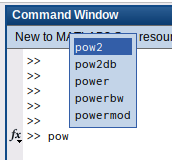
\includegraphics[width=100pt]{images/commandtab}
			\caption{Command Window Sugesti}
		\end{figure}

		Silahkan pilih dengan tombol \keys{$\uparrow$} dan \keys{$\downarrow$}.
		Tekan ENTER (\keys{\return}) untuk eksekusi pilihan.

		\item \textbf{History}.
		Jika ingin mengulang perintah yang sama atau telah dimasukkan sebelumnya,
		ada cukup klik dekat dekat tanda Prompt di Command Window, kemudian tekan tombol panah atas (\keys{$\uparrow$})

		\begin{figure}[!ht]
			\centering
			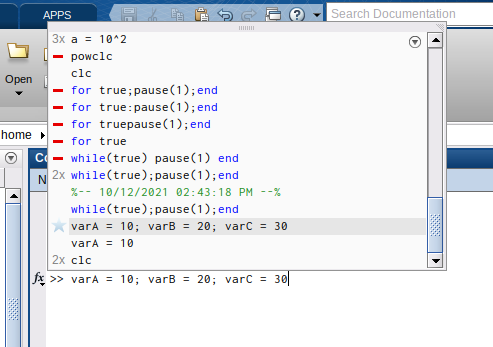
\includegraphics[width=200pt]{images/commandhistory}
			\caption{Command Window History}
		\end{figure}

		Akan muncul history perintah yang pernah dimasukkan.
		Anda tinggal pilih dengan tombol panah atas (\keys{$\uparrow$}) dan panah bawah (\keys{$\downarrow$}).
		Tekan ENTER (\keys{\return}) untuk mengeksekusi perintah yang dipilih.

	\end{itemize}

	\subsection{Ready Indicator}

	Bagian ini menunjukkan siap tidaknya MATLAB untuk menerima perintah.
	Kemungkinan nilai yang muncul:
	\begin{itemize}
		\item \textbf{Busy}. Menandakan MATLAB sedang sibuk dan tidak bisa menerima perintah.
		\item \textbf{Ready}. Menandakan MATLAB siap menerima perintah setelah start-up.
		\item \textbf{Tidak ada label}. Menandakan MATLAB siap menerima perintah.
	\end{itemize}

	\subsection{Workspace}

	Workspace adalah tempat semua variable yang bersifat global ditampilkan.
	Disini kita dapat melihat nilai suatu variable, ukuran dan nilai array, serta variable yang di-import.

	Sebagai contoh jika kita masukkan perintah:
	\begin{minted}[frame=lines,framesep=2mm,fontsize=\small,bgcolor=LightGray]{matlab}
>> varA = 10; varB = 20; varC = 30
	\end{minted}

	\newpage
	Maka tampil di Workspace:

	\begin{figure}[!ht]
		\centering
		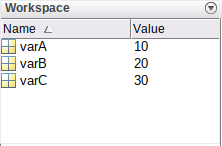
\includegraphics[width=150pt]{images/workspace}
		\caption{Variabel di Workspace}
	\end{figure}

	Untuk membersihkan Workspace, masukkan perintah berikut di Command Window
	\begin{minted}[frame=lines,framesep=2mm,fontsize=\small,bgcolor=LightGray]{matlab}
>> clear
	\end{minted}

	\subsection{Editor}
	Editor adalah bagian MATLAB yang digunakan untuk menulisan skrip yang dapat dieksekusi oleh MATLAB.
	Skrip pada dasarnya adalah kumpulan perintah-perintah MATLAB (dapat dieksekusi di Command Window),
	yang kemudian dieksekusi secara berurutan dari baris atas ke bawah dari file skrip.

	Sebagai contoh, masukkan perintah-perintah berikut ke Editor (bukan Command-Window)
	\begin{minted}[frame=lines,framesep=2mm,fontsize=\small,bgcolor=LightGray]{matlab}
clear;
clc;

varA = 10;
varB = 20;
varC = 30;
	\end{minted}

	Klik icon \textit{Save} pada toolbar tab \textit{Editor} dengan nama file berektensi \textbf{*.m}.

	\begin{figure}[!ht]
		\centering
		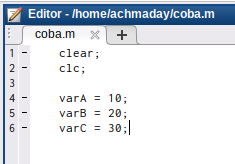
\includegraphics[width=175pt]{images/editorcoba}
		\caption{Contoh Skrip pada Editor}
	\end{figure}

	Selanjutnya, klik icon \textit{Run} (panah segitiga hijau) pada toolbar tab \textit{Editor} untuk menjalankan skrip.

	Atau dapat pula dipanggil melalui Command Window dengan memasukkan nama file skrip tanpa ekstensi.
	Contoh jika skrip disimpan sebagai \textbf{coba.m}, maka perintah untuk memanggil skrip:
	\begin{minted}[frame=lines,framesep=2mm,fontsize=\small,bgcolor=LightGray]{matlab}
>> coba
	\end{minted}

	\textbf{TIPS:} Topik file skrip dan file fungsi lebih jauh akan dibahas pada bab selanjutnya.\\

	\newpage
	\chapter{Pemrograman Dasar}

	Bab ini menjelaskan tutorial pemrograman dasar MATLAB.
	Untuk dapat mengikuti panduan ini, diasumsikan bahwa telah familiar dengan antar-muka MATLAB sebagaimana dijelaskan bab sebelumnya.
	Terutama bagian Command-Window karena panduan ini akan berfokus menggunakan Command-Window.

	\section{Operator}

	\subsection{Matematika Dasar}

	Berikut operator dasar matematika:

	\begin{center}
		\begin{tabular}{|c|c|}
			\hline
			Operator & Makna \\
			\hline\hline
			+ & Penambahan \\
			\hline
			- & Pengurangan \\
			\hline
			* & Perkalian \\
			\hline
			/ & Pembagian \\
			\hline
			\char`\^ & Pangkat \\
			\hline
		\end{tabular}
	\end{center}

	\textbf{PERHATIAN:} Simbol "\textbf{/}" (pembagi) dan "\textbf{\textbackslash}" (linear solver) memiliki makna yang jauh berbeda.
	Harap diperhatikan.

	Contoh:
	\begin{minted}[frame=lines,framesep=2mm,fontsize=\small,bgcolor=LightGray]{matlab}
>> 10^2
ans =
    100
	\end{minted}

	\textbf{TIPS:} variable \textbf{ans} (singkatan dari answer), adalah variabel output default jika tidak ada assigment variable dalam statement.
	Anda dapat menggunakan variable \textbf{ans} untuk operasi selanjutnya

	Contoh:
	\begin{minted}[frame=lines,framesep=2mm,fontsize=\small,bgcolor=LightGray]{matlab}
>> 10^2
ans =
    100

>> ans^2
ans =
    10000
	\end{minted}
	\\

	Untuk urutan operasi dalam satu baris, tetap mengikuti kaidah priotias dimana operasi pangkat didahulukan, diikuti perkalian dan pembagian, kemudian tambah dan kurang.
	Namun urutan ini juga dapat di override menggunakan tanda kurung.

	Contoh:
	\begin{minted}[frame=lines,framesep=2mm,fontsize=\small,bgcolor=LightGray]{matlab}
>> 8+2^2
ans =
    12

>> 8+4*2^2
ans =
    24

>> (8+2)^2
ans =
    100
	\end{minted}

	Sedangkan untuk operasi di luar perhitungan aritmatik (semisal trigonometri, logaritma, sisa pembagian, akar, dst), tidak menggunakan operator khusus.
	Melainkan menggunakan fungsi-fungsi yang tersedia di MATLAB.

	Contoh Trigonometri (Radiant):
	\begin{minted}[frame=lines,framesep=2mm,fontsize=\small,bgcolor=LightGray]{matlab}
>> sin(0.5*pi)
ans =
    1

>> tan(0.5*pi)
ans =
    1.6331e+16
	\end{minted}

	\textbf{TIPS:} Notasi angka dengan \textbf{A.BBe+C} atau \textbf{A.BBe-C} adalah bentuk notasi saintifik.
	Equivalen dengan bentuk $A.BB x 10^C$ atau $A.BB x 10^{-C}$.
	Untuk contoh fungsi \textbf{tan()} di atas, notasi saintifik hasilnya adalah (\textbf{$1.6331x10^{16}$}).\\

	\textbf{TIPS:} Implementasi Trigonometri di MATLAB pada dasarnya menggunakan pendekatan deret Taylor.
	Untuk itu, beberapa fungsi seperti \textbf{tan(pi/2)} seperti di atas memberikan nilai yang sangat besar (mencapai $10^{16}$)
	alih-alih nilai tak berhingga sebagaimana kaidah umum Trigonometry.

	\subsection{Variabel Dasar}

	Variabel adalah identifier dalam pemrograman yang digunakan untuk menyimpan suatu nilai.
	Seluruh pengolahan dan perhitungan dalam MATLAB umumnya dilakukan pada variabel.

	Untuk membuat variable, anda cukup melakukan assignment:
	\begin{minted}[frame=lines,framesep=2mm,fontsize=\small,bgcolor=LightGray]{matlab}
>> varA = 10;
	\end{minted}

	Anda juga dapat membuat variable dari hasil fungsi atau perhitungan
	\begin{minted}[frame=lines,framesep=2mm,fontsize=\small,bgcolor=LightGray]{matlab}
>> varB = 8^2; varC = sin(pi/2);
	\end{minted}

	Variable yang ada buat akan tampil di Workspace, atau dapat dilihat dengan perintah:
	\begin{minted}[frame=lines,framesep=2mm,fontsize=\small,bgcolor=LightGray]{matlab}
>> whos
	\end{minted}

	\newpage
	Anda juga dapat melihat isi variable dengan memanggil nama variabel tersebut
	\begin{minted}[frame=lines,framesep=2mm,fontsize=\small,bgcolor=LightGray]{matlab}
>> varA
varA =
     10
	\end{minted}

	Dengan konsep variabel, anda dapat melakukan kalkulasi dengan nilai yang berubah-ubah sesuai proses kalkulasi namun dengan nama identifier tetap.
	\begin{minted}[frame=lines,framesep=2mm,fontsize=\small,bgcolor=LightGray]{matlab}
>> varA = varB + varC
varA =
     65
	\end{minted}

	\textbf{PERHATIAN:} Beberapa aturan dalam membuat nama variabel atau fungsi:
	\begin{itemize}
		\item Terdiri dari kombinasi alphanumeric (a-z, A-Z, dan 0-9) dan underscore (\_)
		\item Karakter pertama hanya boleh huruf, tidak boleh angka dan tidak boleh underscore.
		\item Tidak boleh memakai titik (\textbf{.}) karena simbol titik adalah operator yang memiliki arti sendiri (untuk data struktur)
		\item Tidak boleh memakai spasi karena spasi adalah pemisah identifier.
		Jika butuh dua kata untuk nama variable, dapat menggunakan:
		\begin{enumerate}
			\item pemisah undescore (\_), contoh: var\_Baru, var\_Lama, dst
			\item camel-case, contoh: varBaru, varLama
		\end{enumerate}
		\item Gunakan nama variabel yang ringkas dan mudah diingat.
	\end{itemize}

	\subsection{Operasi Logika}

	Berikut adalah pembahasan operator logika dimana kalkulasi dilakukan ke variable boolean.
	Variable Boolean adalah variable yang hanya memiliki nilai benar (\textbf{true}) atau salah (\textbf{false}).
	Nilai \textbf{true} setara dengan nilai 1 dan \textbf{false} setara dengan 0.
	Operasi Logika akan sangat bermanfaat nanti untuk topik kendali \textbf{if} dan perulangan \textbf{loop}.

	\begin{itemize}
		\item \textbf{not (\textasciitilde)}. Untuk membalik atau negasi nilai boolean.
		\begin{minted}[frame=lines,framesep=2mm,fontsize=\small,bgcolor=LightGray]{matlab}
>> A = true
A =
  1

>> ~A
ans =
   0

>> not(A)
ans =
   0
		\end{minted}

		\newpage
		\item \textbf{and (\&)}. Untuk membandingkan dua nilai boolean dimana akan bernilai benar jika keduanya benar.
		\begin{minted}[frame=lines,framesep=2mm,fontsize=\small,bgcolor=LightGray]{matlab}
>> A = true; B = true;
>> A & B
ans =
    1

>> and(A,B)
ans =
    1

>> and(A, ~B)
ans =
    0
		\end{minted}

		\item \textbf{or (|)}. Untuk membandingkan dua nilai boolean dimana akan bernilai benar jika salah satu benar.
		\begin{minted}[frame=lines,framesep=2mm,fontsize=\small,bgcolor=LightGray]{matlab}
>> A = true; B = true;
>> A | B
ans =
    1

>> or(A,B)
ans =
    1

>> or(A, ~B)
ans =
    1
		\end{minted}
	\end{itemize}

	\section{Vektor/Matrix}

	Bagian ini akan membahas topik terkait Vektor dan Matrix.
	Pada dasarnya, Vektor/Matrix adalah variable sama seperti sebelumnya,
	namun dalam satu variable berisi lebih dari satu nilai.

	\subsection{Vektor}

	Vektor adalah jenis variable yang berisi beberapa nilai (atau disebut juga elemen).
	Vektor memiliki dimensi 1xN, dimana N adalah jumlah nilai/elemen yang dimiliki.

	\subsubsection{Membuat Vektor}

	Untuk membuat vektor, anda dapat mendaftar setiap elemen dengan dibatasi kurung siku dan dipisah oleh spasi atau koma.
	\begin{minted}[frame=lines,framesep=2mm,fontsize=\small,bgcolor=LightGray]{matlab}
>> w = [0,3,5,1,2,8]
w =
  0 3 5 1 2 8
	\end{minted}

	\textbf{TIPS:} Anda selalu dapat melihat ukuran (bukan nilai) variable global di Workspace atau dengan perintah \textbf{whos}.\\

	Jika vektor yang dibuat teratur dengan interval 1, anda dapat gunakan operator colon (:) seperti:
	\begin{minted}[frame=lines,framesep=2mm,fontsize=\small,bgcolor=LightGray]{matlab}
variabel = awal:akhir
	\end{minted}

	Contoh:
	\begin{minted}[frame=lines,framesep=2mm,fontsize=\small,bgcolor=LightGray]{matlab}
>> w = 0:5
w =
  0 1 2 3 4 5
	\end{minted}

	Jika vektor yang dibuat teratur dengan interval tertentu (bukan 1), anda dapat gunakan operator colon:
	\begin{minted}[frame=lines,framesep=2mm,fontsize=\small,bgcolor=LightGray]{matlab}
variabel = awal:interval:akhir
	\end{minted}

	Contoh:
	\begin{minted}[frame=lines,framesep=2mm,fontsize=\small,bgcolor=LightGray]{matlab}
>> w = -2:3:8
w =
  -2 1 4 7
	\end{minted}

	\subsubsection{Fungsi Linspace}

	Selain menggunakan metode manual dan operator colon, anda juga dapat menggunakan fungsi untuk membuat vektor.
	Contoh salah satu yang banyak dipakai adalah fungsi \textbf{linspace()}.

	Fungsi linspace() (linearly spaced) digunakan untuk membuat vektor pada sejumlah elemen tertentu dengan selisih konstan.
	Perbedaan dengan operator colon adalah pada linspace yang diatur adalah jumlah elemen, sedangkan operator colon yang diatur adalah intervalnya.
	Perintah fungsi linspace():
	\begin{minted}[frame=lines,framesep=2mm,fontsize=\small,bgcolor=LightGray]{matlab}
>> variabel = linspace(awal,akhir,banyaknya)
	\end{minted}

	Jika jumlah elemen tidak dicantumkan maka secara default fungsi linspace() akan membuat vektor 100 elemen.

	Contoh:
	\begin{minted}[frame=lines,framesep=2mm,fontsize=\small,bgcolor=LightGray]{matlab}
>> w = linspace(0,2,4)
w =
  0 0.6667 1.3333 2.000
	\end{minted}

	Jika nilai awal dan akhir sama, maka fungsi linspace akan membuat vektor bernilai sama sejumlah elemen yang ditentukan.
	\begin{minted}[frame=lines,framesep=2mm,fontsize=\small,bgcolor=LightGray]{matlab}
>> w = linspace(2,2,4)
w =
  2 2 2 2
	\end{minted}

	\textbf{TIPS:} Untuk fungsi linspace() dengan nilai awal dan akhir berbeda, maka operator colon yang equivalen:
	\begin{minted}[frame=lines,framesep=2mm,fontsize=\small,bgcolor=LightGray]{matlab}
>> variabel = awal:(akhir-awal)/(jumlah-1):akhir
	\end{minted}

	\newpage
	Contoh:
	\begin{minted}[frame=lines,framesep=2mm,fontsize=\small,bgcolor=LightGray]{matlab}
>> w = 0:(2-0)/(4-1):2
w =
  0 0.6667 1.3333 2.000
	\end{minted}

	\subsubsection{Index Vektor}

	Index adalah urutan suatu elemen dalam suatu vektor.
	Index di MATLAB selalu dimulai dari angka 1.
	Dengan menggunakan index, kita dapat mengakses nilai elemen secara spesifik sesuai urutan.

	Contoh mengakses elemen ke 3 dari vektor sebelumnya:
	\begin{minted}[frame=lines,framesep=2mm,fontsize=\small,bgcolor=LightGray]{matlab}
>> w = linspace(0,2,4);
>> w(3)
ans =
    1.3333
	\end{minted}

	Anda juga dapat mengganti nilai suatu elemen dengan index tersebut.
	\begin{minted}[frame=lines,framesep=2mm,fontsize=\small,bgcolor=LightGray]{matlab}
>> w(3) = 5
w =
  0 0.6667 5.0000 2.0000
	\end{minted}

	Selain satu elemen, anda dapat juga seleksi sejumlah elemen dengan operator colon.
	\begin{minted}[frame=lines,framesep=2mm,fontsize=\small,bgcolor=LightGray]{matlab}
>> variabel(awal:interval:akhir)
	\end{minted}

	Contoh untuk memilih nilai urutan ke-2 hingga ke-4:
	\begin{minted}[frame=lines,framesep=2mm,fontsize=\small,bgcolor=LightGray]{matlab}
>> w = 20:-1:0;
>> w(2:4)
w =
  18 16 14
	\end{minted}

	Anda juga dapat memilih hanya bilangan genap dengan memilih urutan pertama yang merupakan bilangan genap,
	kemudian urutan interval bernilai 2.

	Contoh memilih bilangan genap dari urutan ke-3 hingga ke-9
	\begin{minted}[frame=lines,framesep=2mm,fontsize=\small,bgcolor=LightGray]{matlab}
>> w = 20:-1:0;
>> w(3:2:9)
w =
  18 16 14 12
	\end{minted}

	Untuk memilih bilangan ganjil, anda tinggal memilih bilangan ganjil pertama dan terakhir, namun interval tetep bernilai 2.
	\begin{minted}[frame=lines,framesep=2mm,fontsize=\small,bgcolor=LightGray]{matlab}
>> w = 20:-1:0;
>> w(4:2:10)
w =
  17 15 13 11
	\end{minted}

	\newpage
	\subsubsection{Operasi Vektor}

	Vektor juga dapat dioperasikan sebagaimana variabel.
	Bahkan variabel dengan satu nilai (skalar) pada hakikatnya adalah vektor berukuran 1x1.
	Operasi pada vektor dapat dilakukan per elemen atau sebagai seluruh vektor.

	Berikut tabel operasi per elemen antara dua vektor:
	\begin{center}
		\begin{tabular}{|c|c|c|}
			\hline
			Operator Skalar & Makna & Operasi Vektor Per-Elemen\\
			\hline\hline
			+ & Penambahan & +  \\
			\hline
			- & Pengurangan & - \\
			\hline
			* & Perkalian & .* \\
			\hline
			/ & Pembagian & ./ \\
			\hline
			\char`\^ & Pangkat & .\char`\^   \\
			\hline
		\end{tabular}
	\end{center}

	\textbf{PERHATIAN:} Untuk semua operasi di tabel di atas, kedua vektor harus memiliki dimensi yang sama.\\

	Contoh:
	\begin{minted}[frame=lines,framesep=2mm,fontsize=\small,bgcolor=LightGray]{matlab}
>> v = [2,4,6]; w = [1,3,5];
>> v+w
ans =
    3 7 11

>> v-w
ans =
    1 1 1

>> v.*w
ans =
    2 12 30

>> v./w
ans =
    2.0000 1.3333 1.2000

>> v.^2
ans =
    4 16 36
	\end{minted}

	\subsubsection{Transpose}

	Untuk melakukan operasi Transpose vektor (menukar kolom dan baris), digunakan tanda aposthrope (').
	Contoh:
	\begin{minted}[frame=lines,framesep=2mm,fontsize=\small,bgcolor=LightGray]{matlab}
>> w = linspace(0,2,4)
w =
  0 0.6667 1.3333 2.0000

>> wT = w'
wT =
   0
   0.6667
   1.3333
   2.0000
	\end{minted}

	\newpage
	\subsubsection{Vector Multiplication}

	Dengan menggunakan operasi Transpose, ada dapat mengkalikan dua vektor (bukan per elemen),
	dengan kaidah matematika perkalian matrix, dimana baris vektor terkali harus sama dengan jumlah kolom matrix pengali.
	\\
	Untuk itu, jika diperlukan, matrix pengali harus di transpose.
	Hasil perkalian dua vektor akan menghasilkan satu nilai skalar.

	\[
	\begin{bmatrix}
		a_1 & a_2 & a_3
	\end{bmatrix}
	.
	\begin{bmatrix}
		b_1 \\
		b_2 \\
		b_3
	\end{bmatrix}
	=
	a_{1}b_{1} + a_{2}b_{2} + a_{3}b_{3}
	\]

	\textbf{PERHATIAN:} Dalam kaidah perkalian matrix, kaidah komutatif tidak berlaku.
	Sementara kaidah asosiatif dan distributif secara umum masih berlaku.

	Contoh:
	\begin{minted}[frame=lines,framesep=2mm,fontsize=\small,bgcolor=LightGray]{matlab}
>> v = [2,4,6]; w = [1,3,5];
>> v*w
Error

>> v*w'
ans =
    44

>> w*v'
ans =
    44
	\end{minted}

	Perhitungan di atas adalah \textbf{2x1 + 4x3 + 5x6 = 44}.
	Hasil perkalian satu nilai skalar sehingga membalik terkali dan transpose pengali akan menghasilkan nilai sama.
	Namun perkalian antara transpose terkali dan pengali akan menghasilkan matrix yang berbeda (kaidah komutatif tidak berlaku).

	\subsection{Matrix}

	Matrix adalah vektor dengan dimensi MxN, dengan $M,N \geq 1$

	\subsubsection{Membuat Matrix}

	Untuk membuat matrix, anda dapat mendaftar setiap elemen dengan dibatasi kurung siku dan dipisah oleh spasi atau koma.
	Kemudian setiap baris dipisah oleh semi-colon (;).
	\begin{minted}[frame=lines,framesep=2mm,fontsize=\small,bgcolor=LightGray]{matlab}
>> w = [0,3,5; 1,2,8; 5,7,9]
w =
  0 3 5
  1 2 8
  5 7 9
	\end{minted}

	Anda juga dapat menggunakan operator colon seperti pada vektor:
	\begin{minted}[frame=lines,framesep=2mm,fontsize=\small,bgcolor=LightGray]{matlab}
>> w = [0:1:2; 4:1:6; 5:1:7]
w =
  0 1 2
  4 5 6
  5 6 7
	\end{minted}

	\textbf{PERHATIAN:} Pastikan jumlah elemen setiap baris harus sama.

	\subsubsection{Fungsi Matrix}

	Selain menggunakan metode manual dan operator colon, anda juga dapat menggunakan fungsi untuk membuat matrix.
	Beberapa fungsi yang umum dipakai antara lain:
	\begin{itemize}
		\item \textbf{zeros()}. Fungsi zeros() dipakai untuk membuat matrix dengan semua nilai 0.

		Contoh membuat matrix 0 berukuruan 3x3:
		\begin{minted}[frame=lines,framesep=2mm,fontsize=\small,bgcolor=LightGray]{matlab}
>> w = zeros(3)
w =
  0 0 0
  0 0 0
  0 0 0
		\end{minted}

		Contoh membuat matrix 0 berukuran 3x2:
		\begin{minted}[frame=lines,framesep=2mm,fontsize=\small,bgcolor=LightGray]{matlab}
>> w = zeros(3,2)
w =
  0 0
  0 0
  0 0
		\end{minted}

		\item \textbf{ones()}. Fungsi one() sama dengan zeros namun dipakai untuk membuat matrix dengan semua nilai 1.
		\begin{minted}[frame=lines,framesep=2mm,fontsize=\small,bgcolor=LightGray]{matlab}
>> w = ones(3)
w =
  1 1 1
  1 1 1
  1 1 1

>> w = ones(3,2)
w =
  1 1
  1 1
  1 1
		\end{minted}

		\item \textbf{rand()},\textbf{randi()}, dan \textbf{randn()}. Ketiga fungsi ini digunakan untuk membuat matrix berisi bilangan random.
		Contoh rand() yang menggunakan uniform distribution randomization. Input adalah ukuran matrix persegi yang diinginkan:
		\begin{minted}[frame=lines,framesep=2mm,fontsize=\small,bgcolor=LightGray]{matlab}
>> w = rand(2)
w =
  0.9595 0.0357
  0.6557 0.8491
		\end{minted}

		Contoh randi() dimana sama dengan rand() namun hasilnya integer. Input adalah bilangan maksimal dan ukuran matrix persegi yang diinginkan:
		\newpage
		\begin{minted}[frame=lines,framesep=2mm,fontsize=\small,bgcolor=LightGray]{matlab}
>> w = randi(10,2)
w =
  10 8
  7  3
	\end{minted}

	Contoh randn() dimana sama dengan rand() namun menggunakan normal distribution randomization sehingga ada nilai negatif.
	Input adalah ukuran matrix persegi yang diinginkan:
	\begin{minted}[frame=lines,framesep=2mm,fontsize=\small,bgcolor=LightGray]{matlab}
>> w = randn(2)
w =
 -0.3034 -0.7873
  0.2939  0.8884
	\end{minted}

	\end{itemize}

	\subsubsection{Concatenate}

	Untuk membuat matrix, anda juga dapat lakukan dengan menyatukan (concatenate) dua atau lebih vektor/matrix menggunakan tanda kurung (\textbf{[]})

	Contoh menyatukan dua vektor secara horizontal, dipisah oleh tanda koma
	\begin{minted}[frame=lines,framesep=2mm,fontsize=\small,bgcolor=LightGray]{matlab}
>> u = [0,1,2] v = [4,5,6];
>> w = [u,v]
w =
  0 1 2 4 5 6
	\end{minted}

	Contoh menyatukan dua vektor secara vertical, dipisah oleh tanda semi-colon
	\begin{minted}[frame=lines,framesep=2mm,fontsize=\small,bgcolor=LightGray]{matlab}
>> u = [0,1,2] v = [4,5,6];
>> w = [u;v]
w =
  0 1 2
  4 5 6
	\end{minted}

	\textbf{PERHATIAN:} Untuk menyatukan dua vektor/matrix pastikan dimensinya kompatibel.
	Jika menyatukan horizontal, maka dimensi baris harus sama.
	Untuk vertikal, maka dimensi kolom harus sama.
	\subsubsection{Index Matrix}

	Akses elemen pada matrix juga sama seperti vektor dengan menggunakan index.
	Perbedaannya adalah index terdiri dari 2 angka terpisah koma yang masing-masing menunjukkan urutan baris dan kolom.

	Contoh elemen pada baris 2 dan kolom 2:
	\begin{minted}[frame=lines,framesep=2mm,fontsize=\small,bgcolor=LightGray]{matlab}
>> w = [0,3,5; 1,4,8; 5,7,9];
>> w(2,2)
ans =
    4
	\end{minted}

	\textbf{PERHATIAN:} angka pertama pada index selalu adalah baris dan angka kedua adalah kolom.\\

	Sama seperti vektor, element juga dapat diubah nilainya dengan index:
	\begin{minted}[frame=lines,framesep=2mm,fontsize=\small,bgcolor=LightGray]{matlab}
>> w = [0,3,5; 1,4,8; 5,7,9];
>> w(2,2)=11
w =
  0  3 5
  1 11 8
  5  7 9
	\end{minted}

	Berlaku juga operator colon (:) untuk memilih sebagian isi matrix
	Contoh memilih baris 2 sampai 3 dan kolom 3 sampai 5:
	\begin{minted}[frame=lines,framesep=2mm,fontsize=\small,bgcolor=LightGray]{matlab}
>> w = [0,3,5,6,11; 1,4,8,7,4; 5,7,9,8,10; 2,10,16,8,5; 9,0,6,4,3];
>> w(2:3,3:5)
ans =
    8 7 4
    9 8 10
	\end{minted}

	Untuk memilih seluruh baris atau kolom, cukup ganti angka dengan operator colon (:).
	Contoh memilih seluruh kolom pada baris ke-3
	\begin{minted}[frame=lines,framesep=2mm,fontsize=\small,bgcolor=LightGray]{matlab}
>> w = [0,3,5,6,11; 1,4,8,7,4; 5,7,9,8,10; 2,10,16,8,5; 9,0,6,4,3];
>> w(3,:)
ans =
    5 7 9 8 10
	\end{minted}

	Contoh memilih seluruh baris pada baris ke-2
	\begin{minted}[frame=lines,framesep=2mm,fontsize=\small,bgcolor=LightGray]{matlab}
>> w = [0,3,5,6,11; 1,4,8,7,4; 5,7,9,8,10; 2,10,16,8,5; 9,0,6,4,3];
>> w(:,2)
ans =
    3
    4
    7
   10
    0
	\end{minted}

	\subsubsection{Determinant/Inverse}

	Dalam kaidah matrix, sebuah matrix persegi memiliki kebalikan atau inverse matrix.
	Contoh untuk matrix 2x2:

	\[
	\begin{bmatrix}
		a & b\\
		c & d
	\end{bmatrix}^{-1}
	=
	\frac{1}{ad-bc}
	\begin{bmatrix}
		d & -b \\
		-c & a\\
	\end{bmatrix}
	\]

	dimana nilai $ad-bc$ disebut Determinant.
	Jika suatu matrix dikalikan dengan inverse matrixnya:

	\[
	\begin{bmatrix}
		a & b\\
		c & d
	\end{bmatrix}
	\begin{bmatrix}
		a & b\\
		c & d
	\end{bmatrix}^{-1}
	=
	\frac{1}{ad-bc}
	\begin{bmatrix}
		a & b\\
		c & d
	\end{bmatrix}
	\begin{bmatrix}
		d & -b \\
		-c & a\\
	\end{bmatrix}
	=
	\frac{1}{ad-bc}
	\begin{bmatrix}
		ad-bc & -ab+ba\\
		cd-dc & -bc+da
	\end{bmatrix}
	=
	\begin{bmatrix}
		1 & 0\\
		0 & 1
	\end{bmatrix}
	\]

	Maka didapat matrix identitas (atau biasa disebut \textbf{I}).

	Untuk mendapatkan nilai determinant dan inverse di MATLAB, digunakan fungsi \textbf{det()} dan \textbf{inv()}.

	Contoh:
	\begin{minted}[frame=lines,framesep=2mm,fontsize=\small,bgcolor=LightGray]{matlab}
>> A = [4,2;3,5];
>> dA = det(A)
dA =
   14

>> invA = inv(A)
invA =
     0.3571 -0.1429
    -0.2143 -0.2857

>> invA.*dA
ans =
    5 -2
   -3  4
	\end{minted}

	Terlihat bahwa matrix \textbf{invA} adalah inversi dari matrik A, yang jika dikalikan kedua akan menghasilkan matrix identitas:
	\begin{minted}[frame=lines,framesep=2mm,fontsize=\small,bgcolor=LightGray]{matlab}
>> A*invA
ans =
    1.0000     0
    0     1.0000
	\end{minted}

	\textbf{TIPS:} Anda juga dapat menggunakan fungsi \textbf{eye()} untuk membuat matrix identitas dengan input ukuran matrix persegi:
	 \begin{minted}[frame=lines,framesep=2mm,fontsize=\small,bgcolor=LightGray]{matlab}
I = eye(2)
ans =
    1 0
    0 1
	 \end{minted}

	\section{Format Angka}
	\subsection{Pecahan}

	Untuk mengubah format jumlah angka decimal pada MATLAB, digunakan perintah \textbf{format}.

	\begin{center}
		\begin{tabular}{|c|c|}
			\hline
			Format & Makna \\
			\hline\hline
			short & 4 angka decimal \\
			\hline
			long & 14 angka decimal \\
			\hline
			bank & 2 angka decimal \\
			\hline
			rat & bentuk fraksi pecahan \\
			\hline
		\end{tabular}
	\end{center}

	Contoh:
	\begin{minted}[frame=lines,framesep=2mm,fontsize=\small,bgcolor=LightGray]{matlab}
>> format short
>> sqrt(5)
ans =
    2.2361

>> format long
>> sqrt(5)
and =
    2.236067977499790

>> format bank
>> sqrt(5)
ans =
    2.24

>> format rat
>> sqrt(5)
ans =
    2889/1292
	\end{minted}

    Secara default, MATLAB memilih \textbf{short} saat startup.
    Pengaturan tampilan tidak mempengaruhi nilai aktual yang disimpan dan memory MATLAB.

    \textbf{TIPS:} Untuk mengembalikan ke default, masukkan \textbf{format short} atau \textbf{format} saja.

    \subsection{Pembulatan}

    Tersedia beberapa fungsi pembulatan yang dapat digunakan:

    \begin{center}
    	\begin{tabular}{|c|c|}
    		\hline
    		Fungsi & Makna \\
    		\hline\hline
    		round & Mendekati integer\\
    		\hline
    		ceil & Mendekati integer arah positif tak hingga \\
    		\hline
    		floor & Mendekati integer arah negatif tak hingga \\
    		\hline
    		fix & Mendekati integer arah angka nol \\
    		\hline
    	\end{tabular}
    \end{center}

	Contoh:
	\begin{minted}[frame=lines,framesep=2mm,fontsize=\small,bgcolor=LightGray]{matlab}
>> 53/7
ans =
    7.5714

>> round(53/7)
ans =
    8

>> fix(53/7)
ans =
    7
	\end{minted}

	\subsection{Kompleks}

	Bilangan kompleks adalah bilangan yang melibatkan nilai $\sqrt{-1}$ yang disimbolkan sebagai \textbf{i}.
	Bilangan ini hadir sebagai solusi persamaan $x^{2}+1=0$.
	Terdiri dari 2 bagian, real dan imaginer yang biasa ditulis $\Re+\Im i$.
	Beberapa bentuk penulisan bilangan kompleks di MATLAB
	\begin{minted}[frame=lines,framesep=2mm,fontsize=\small,bgcolor=LightGray]{matlab}
>> C = 3-2i;
>> C = 3-2*i;
>> C = 3-2*sqrt(-1)
>> C = complex(3,-2)
	\end{minted}

	Tersedia pula beberapa fungsi berkaitan bilangan kompleks.
	\begin{itemize}
		\item \textbf{conj()}. Untuk mendapatkan nilai konjugasi
		\begin{minted}[frame=lines,framesep=2mm,fontsize=\small,bgcolor=LightGray]{matlab}
>> C = 3-2i;
>> conj(C)
ans =
    3.0000 + 2.0000i
		\end{minted}

		\item \textbf{real()} dan \textbf{imag()}. Untuk mendapatkan masing-masing bilang real dan imaginer.
		\begin{minted}[frame=lines,framesep=2mm,fontsize=\small,bgcolor=LightGray]{matlab}
>> C = 3-2i;
>> real(C)
ans =
    3

>> imag(C)
ans =
    -2
		\end{minted}

		\item \textbf{abs()} dan \textbf{angle()}. Untuk mendapatkan masing-masing magnitude (absolute) dan sudut-fase.
		\begin{minted}[frame=lines,framesep=2mm,fontsize=\small,bgcolor=LightGray]{matlab}
>> C = 3-2i;
>> real(C)
ans =
    3.6065

>> imag(C)
ans =
    -0.5880
		\end{minted}
	\end{itemize}

	\section{Struct Array}

	Array Struktur adalah jenis variabel yang merupakan suatu grup dari beberapa variabel.
	Variabel anggota grup dapat diakses dengan operator titik (\textbf{.}).
	Setiap variabel anggota grup disebut sebagai \textbf{field}.
	Variabel jenis ini dapat dideklarasikan dengan fungsi \textbf{struct()}.
	Nama field dideklarasikan dengan diapit petik satu (\textbf{'}).
	\begin{minted}[frame=lines,framesep=2mm,fontsize=\small,bgcolor=LightGray]{matlab}
variabel = struct('field1',value1,'field2',value2,..., 'fieldN',valueN);
	\end{minted}

	Sebagai contoh suatu variabel array struktur berisi vektor dan matrix di field terpisah.
	\begin{minted}[frame=lines,framesep=2mm,fontsize=\small,bgcolor=LightGray]{matlab}
>> w = struct('a',[1,3,5],'b',[2,4,6;8,9,0]);
>> w.a
ans =
    1 3 5
>> w.b
ans =
    2 4 6
    8 9 0
	\end{minted}

	\newpage
	Selain dengan fungsi struct(), anda juga dapat membuat variabel struct layaknya variabel pada umumnya dengan operator titik (\textbf{.}).
	\begin{minted}[frame=lines,framesep=2mm,fontsize=\small,bgcolor=LightGray]{matlab}
>> s.a = [1,3,6]
s =
  a: [1 3 6]
>> s.b =
s =
  a: [1 3 6]
  b: 'abc'
	\end{minted}

	\newpage
	\section{Penugasan}

	\begin{enumerate}
		\item Selesaikan sistem persamaan linear dua peubah berikut dengan metode matrix pada MATLAB.
		\begin{enumerate}[label=(\alph*)]
			\item
			\begin{align*}
				2x-3y&=8 & x+2y&=-3
			\end{align*}

			\item
			\begin{align*}
				2x-3y&=-13 & x+2y&=4
			\end{align*}

			\item
			\begin{align*}
				2x-y&=7 & x+3y&=14
			\end{align*}
		\end{enumerate}

		\item Selesaikan sistem persamaan linear tiga peubah berikut dengan metode matrix pada MATLAB.
		\begin{enumerate}[label=(\alph*)]
			\item
			\begin{align*}
				2x-3y+2z&=-3 & x+2y+z&=2 & 2x-y+3z&=1
			\end{align*}

			\item
			\begin{align*}
				x+y&=1 & y+z&=3 & z+x&=6
			\end{align*}

			\item
			\begin{align*}
				x-3y+2z&=9 & 2x+4y-3z&=-9 & 3x-2y+5z&=12
			\end{align*}
		\end{enumerate}
	\end{enumerate}

	\newpage
	\chapter{Pemrograman Menengah}

	\section{Symbolic}

	Symbolic adalah salah satu Toolbox di MATLAB yang dapat digunakan untuk operasi matematika secara simbolik dan variabel dinamik.
	Simbolik/Dinamik variabel disini maksudnya adalah variabel tersebut belum memiliki menyimpan nilai tertentu selama proses operasi.
	Secara matematis, disini dilakukan proses aljabar tanpa memperhatikan isi nilai variabel.

	\subsection{Deklarasi}

	Untuk deklarasi simbolik, digunakan perintah \textbf{syms}.
	Deklarasi dilakukan dengan menyebutkan setiap entitas simbol yang dipisah spasi.

	Contoh:
	\begin{minted}[frame=lines,framesep=2mm,fontsize=\small,bgcolor=LightGray]{matlab}
>> syms x y;
	\end{minted}

	Kemudian dapat dibuat persamaan/fungsi dari entitas simbolik.
	Contoh:
 	\begin{minted}[frame=lines,framesep=2mm,fontsize=\small,bgcolor=LightGray]{matlab}
>> z = x^3 - 4*x*y + y^2;
 	\end{minted}

 	Anda juga dapat mencampur variabel skalar dengan simbolik.
 	Contoh:
 	\begin{minted}[frame=lines,framesep=2mm,fontsize=\small,bgcolor=LightGray]{matlab}
>> syms x y;
>> a = 8;
>> z = a^3 - a*x*y + x^2*y
ans =
    y*x^2 - 8*y*x + 512
 	\end{minted}

	\subsection{Operasi}

	Selain mengikuti kaidah aljabar, operasi simbolik juga memiliki fungsi operasi tambahan antara lain:
	\begin{itemize}
		\item \textbf{expand()}. Fungsi ini digunakan untuk menjabarkan suatu persamaan aljabar simbolik.

		Contoh:
		\begin{minted}[frame=lines,framesep=2mm,fontsize=\small,bgcolor=LightGray]{matlab}
>> syms x y;
>> z = (x-y)*(x-y)^2;
>> z = expand(z)
z =
    x^3 - 3*x^2*y + 3*x*y^2 - y^3
		\end{minted}

		\item \textbf{factor()}. Fungsi ini digunakan untuk mendapatkan faktor/akar suatu persamaan aljabar simbolik.
		Fungsi ini kebalikan dari fungsi \textbf{expand()}.
		\begin{minted}[frame=lines,framesep=2mm,fontsize=\small,bgcolor=LightGray]{matlab}
>> syms x y;
>> z = x^3 - 3*x^2*y + 3*x*y^2 - y^3;
>> z = factor(z)
z =
  [x-y, x-y, x-y]
		\end{minted}

		\item \textbf{simplify()}. Fungsi ini untuk menyederhanakan suatu persamaan se-sederhana mungkin.
		Contoh persamaan $sin^{2}(x) + cos^{2}(x) = 1$:
		\begin{minted}[frame=lines,framesep=2mm,fontsize=\small,bgcolor=LightGray]{matlab}
>> syms x;
>> y = sin(x)^2 + cos(x)^2
>> simplify(y)
ans =
    1
		\end{minted}
	\end{itemize}

	Selain aljabar, dapat juga dilakukan operasi kalkulus antara lain:
	\begin{itemize}
		\item \textbf{diff()}. Fungsi diff() digunakan untuk operasi differential pada fungsi simbolik.
		Contoh persamaan sebelumnya diturunkan parsial satu kali terhadap x:
		\begin{minted}[frame=lines,framesep=2mm,fontsize=\small,bgcolor=LightGray]{matlab}
>> syms x y;
>> z = x^3 - 3*x^2*y + 3*x*y^2 - y^3;
>> z1 = diff(z,x)
z1 =
   3*x^2 - 6*x*y + 3*y^2
		\end{minted}

		Dapat pula diturunkan lebih dari satu turunan dengan menambahkan argumen level turunan.
		Contoh persamaan sebelumnya diturunkan parsial dua kali terhadap x:
		\begin{minted}[frame=lines,framesep=2mm,fontsize=\small,bgcolor=LightGray]{matlab}
>> syms x y;
>> z = x^3 - 3*x^2*y + 3*x*y^2 - y^3;
>> z2 = diff(z,x,2)
z2 =
   6*x - 6*y
		\end{minted}

		\item \textbf{int()}. Fungsi int() digunakan untuk operasi integral pada fungsi simbolik.
		Contoh integral persamaan fungsi x:
		\begin{minted}[frame=lines,framesep=2mm,fontsize=\small,bgcolor=LightGray]{matlab}
>> syms x;
>> y = x^2 + 2*x + 3;
>> y0 = int(y)
ans =
    (x*(x^2 + 3*x + 9))/3
>> expand(y0)
ans =
    x^3/3 + x^2 + 3*x
		\end{minted}

		Terlihat tidak ada konstanta tambahan di akhir persamaan hasil integral, karena pada dasarnya fungsi int() digunakan sebagai integral berbatas (definite).
		Sehingga jika batas bawah dan atas suatu integral diketahui, dapat dilakukan integral berbatas dengan hasil akhir skalar.

		Contoh integral persamaan di atas dengan batas bawah 2 dan batas atas 7.
		\begin{minted}[frame=lines,framesep=2mm,fontsize=\small,bgcolor=LightGray]{matlab}
>> syms x;
>> y = x^2 + 2*x + 3;
>> y0 = int(y,2,7)
ans =
    515/3
		\end{minted}

		\item \textbf{symsum()}. Untuk menghitung jumlah deret tak hingga yang konvergen.
		Contoh:
		\[ S = 1 + \frac{1}{2^2} + \frac{1}{3^2} + ... + \frac{1}{n^2}\]

		dengan n tak hingga, maka dalam operasi simbolik yang dimulai dari 1 hingga tak berhingga
		\begin{minted}[frame=lines,framesep=2mm,fontsize=\small,bgcolor=LightGray]{matlab}
>> syms k
>> s = symsum(1/k^2, 1, inf)
s =
  pi^2/6
		\end{minted}

		\item \textbf{limit()}. Untuk menghitung pendekatan limit.
		Contoh:
		\[\lim_{x \to +\infty} \frac{x}{x^2}\]

		Dalam MATLAB:
		\begin{minted}[frame=lines,framesep=2mm,fontsize=\small,bgcolor=LightGray]{matlab}
>> syms x
>> limit(x/x^2, inf)
ans =
    0
		\end{minted}

		\item \textbf{taylor()}. Untuk membentuk expansi deret Taylor dari suatu persamaan.
		Kaidah Taylor series:
		\[f(x) = f(a) + \frac{f'(a)}{1!}(x-a) + \frac{f''(a)}{2!}(x-a)^2 + \frac{f'''(a)}{3!}(x-a)^3 + ...\]

		Secara default, fungsi taylor() menghitung hingga suku ke 5.

		Contoh dalam MATLAB:
		\begin{minted}[frame=lines,framesep=2mm,fontsize=\small,bgcolor=LightGray]{matlab}
>> syms x
>> taylor(sin(x))
ans =
    x^5/120 - x^3/6 + x
		\end{minted}

		Jika butuh suku di atas 5, gunakan keyword field \textbf{'order'}:

		Contoh untuk hingga suku 8:
		\begin{minted}[frame=lines,framesep=2mm,fontsize=\small,bgcolor=LightGray]{matlab}
>> syms x
>> taylor(sin(x),'order',8)
ans =
    -x^7/5040 + x^5/120 - x^3/6 + x
		\end{minted}

	\end{itemize}

	\subsection{Substitusi}

	Jika entitas simbol berada dalam suatu fungsi persamaan, dapat dilakukan substitusi variabel untuk mendapatkan nilai skalar persamaan.
	Fungsi yang digunakan adalah \textbf{subs()}.
	\begin{minted}[frame=lines,framesep=2mm,fontsize=\small,bgcolor=LightGray]{matlab}
>> subs(fungsi, vektor_simbol, vektor_nilai)
	\end{minted}

	Vektor simbol dan vektor nilai haruslah sesuai urutan.

	Contoh:
	\begin{minted}[frame=lines,framesep=2mm,fontsize=\small,bgcolor=LightGray]{matlab}
>> syms a b c x
>> f = a*x^2 + b*x + c
>> subs(f, x, 5)
ans =
    f = a*x^2 + b*x + c

>> subs(f, [a,b,c,x], [1,2,3,5])
ans =
    38
	\end{minted}

	\newpage
	\section{File Kode}

	File kode adalah teks file yang berisi kumpulan perintah-perintah MATLAB untuk dieksekusi secara berurutan oleh MATLAB.
	File kode dapat berupa skrip, fungsi, atau live-script.
	Semua file kode disimpan sebagai file text ASCII dengan ekstensi \textbf{*.m} (bukan *.txt).
	Untuk membuat dan modifikasi file kode, digunakan MATLAB Editor.
	\\
	\\
	\textbf{TIPS:} Selain menggunakan MATLAB Editor, anda dapat menggunakan editor programming lain seperti Notepad++, Visual Studio Code, Atom, Sublime, dst.
	Namun eksekusi file kode tetap dilakukan dalam MATLAB.
	Tidak disarankan menggunakan Notepad bawaan Windows.

	\subsection{Script}

	Skrip adalah format dasar file kode.
	Untuk membuat skrip baru, klik toolbar \textit{HOME} -> \textit{New} -> \textit{Script},
	atau dapat juga \textit{HOME} -> \textit{New Script}.
	MATLAB secara otomatis akan membuka Editor.

	Untuk membuka skrip yang telah disimpan, klik toolbar \textit{HOME} -> \textit{Open}.
	Anda dapat juga menggunakan Current Folder untuk navigasi dan klik dua kali file skrip yang akan dibuka.

	Berikut contoh membuat skrip.
	Buka MATLAB Editor dan masukkan statement-statement berikut:
	\begin{minted}[frame=lines,framesep=2mm,fontsize=\small,bgcolor=LightGray]{matlab}
close all;
clear;

syms x y;

z = x^3 - 3*x^2*y + 3*x*y^2 - y^3;
z1 = diff(z,x);
z2 = diff(z,x,2);

sz = subs(z,[x,y],[2,5]);
sz1 = subs(z1,[x,y],[2,5]);
sz2 = subs(z2,[x,y],[2,5]);

out = "nilai sz: " + string(sz) +...
",sz1: " + string(sz1) +...
",sz2: " + string(sz2);

disp(out);
	\end{minted}

	Simpan dengan klik toolbar di tab \textit{Editor} -> \textit{Save}, simpan dengan nama \textbf{turunan.m}.
	Kemudian eksekusi skrip dengan klik toolbar di tab \textit{Editor} -> \textit{Run}, atau panggil nama skrip (tanpa eksentensi) pada Command-Window:
	\begin{minted}[frame=lines,framesep=2mm,fontsize=\small,bgcolor=LightGray]{matlab}
>> turunan
nilai sz: -27,sz1: 27,sz2: -18
	\end{minted}

	\textbf{Penjelasan}.
	\begin{minted}[frame=lines,framesep=2mm,fontsize=\small,bgcolor=LightGray]{matlab}
close all;
clear;
	\end{minted}

	Baris kode di atas untuk menutup window-window lain (jika ada) dan membersihkan variable yang tersimpan di MATLAB.
	Dengan ini proses kalkulasi dimulai dari kondisi seolah MATLAB selesai start-up.

	\newpage
	Selanjutnya,
	\begin{minted}[frame=lines,framesep=2mm,fontsize=\small,bgcolor=LightGray]{matlab}
syms x y;

z = x^3 - 3*x^2*y + 3*x*y^2 - y^3;
z1 = diff(z,x);
z2 = diff(z,x,2);

sz = subs(z,[x,y],[2,5]);
sz1 = subs(z1,[x,y],[2,5]);
sz2 = subs(z2,[x,y],[2,5]);
	\end{minted}

	Baris kode di atas adalah proses kalkulasi simbolik sebagaimana telah dibahas sebelumnya.

	\begin{minted}[frame=lines,framesep=2mm,fontsize=\small,bgcolor=LightGray]{matlab}
out = "nilai sz: " + string(sz) +...
",sz1: " + string(sz1) +...
",sz2: " + string(sz2);

disp(out)
	\end{minted}

	Baris kode di atas untuk membentuk kalimat yang menampilkan variabel simbol hasil.
	Kemudian ditampilkan dengan fungsi \textbf{disp()}.

	Beberapa hal yang perlu diperhatikan di baris kode tersebut.
	\begin{itemize}
		\item \textbf{String}. String adalah jenis variable yang berisi kata atau kalimat.
		Deklarasi variabel string diapit tanda petik-dobel (").
		Operasi string yang umum digunakan adalah menggabungkan dengan operator penambahan.
		Jika penambahan melibatkan suatu variabel non-string, perlu digunakan fungsi \textbf{string()}, \textbf{num2str()},
		atau yang sejenis untuk konversi string:

		Contoh:
		\begin{minted}[frame=lines,framesep=2mm,fontsize=\small,bgcolor=LightGray]{matlab}
>> nama = "Achmadi";
>> umur = 30;
>> kalimat = "saya " + nama + " berumur " + num2str(umur);
>> disp(kalimat)
saya Achmadi berumur 30
		\end{minted}

		\item \textbf{Tiga-Titik}. Operator Tiga-Titik (\textbf{...}) berguna untuk menyambungkan statement yang berbeda baris
		sehingga seolah dalam satu baris.

		Contoh penjumlahan 10+20+30+40 terpisah satu baris:
		\begin{minted}[frame=lines,framesep=2mm,fontsize=\small,bgcolor=LightGray]{matlab}
>> 10 + 20 + ...
30 + 40
ans =
    100
    	\end{minted}
	\end{itemize}

	\newpage
	\subsection{Fungsi}

	Fungsi adalah perintah yang dapat menerima input dan mengembalikan hasil proses.
	Fungsi terdiri dari empat jenis:
	\begin{enumerate}
		\item \textbf{Built-in}. Fungsi jenis ini telah disediakan oleh instalasi MATLAB.
		Umumnya anda tinggal gunakan dan tidak bisa dimodifikasi oleh pengguna.
		Contoh: Semua fungsi-fungsi yang digunakan sebelum pembahasan ini.

		\item \textbf{Inline}. Fungsi jenis ini menggunakan perintah \textbf{inline()} untuk deklarasi fungsi inline.
		Topik ini dibahas pada bagian selanjutnya.

		\item \textbf{Operator @}. Fungsi jenis ini menggunakan operator @ untuk deklarasi fungsi handler.
		Topik ini dibahas pada bagian selanjutnya.

		\item \textbf{File Fungsi}. Fungsi ini ditulis sebagai file kode seperti skrip.
		Topik ini yang akan dibahas di bagian ini.
	\end{enumerate}

	Template isi file fungsi seperti berikut:
	\begin{minted}[frame=lines,framesep=2mm,fontsize=\small,bgcolor=LightGray]{matlab}
function y = nama_fungsi(x1,x2,x3)
	statement;
end
	\end{minted}

	File fungsi harus disimpan sebagai \textbf{nama\_fungsi.m} sesuai nama fungsi yang dibuat.

	Variasi bentuk fungsi lain:
	\begin{itemize}
		\item Jika output fungsi beberapa variabel
		\begin{minted}[frame=lines,framesep=2mm,fontsize=\small,bgcolor=LightGray]{matlab}
function [y1,y2] = nama_fungsi(x1,x2,x3)
	statement;
end
		\end{minted}

		\item Jika fungsi tidak mengembalikan nilai apapun.
		\begin{minted}[frame=lines,framesep=2mm,fontsize=\small,bgcolor=LightGray]{matlab}
function nama_fungsi(x1,x2,x3)
	statement;
end
		\end{minted}

		\item Jika fungsi tidak memerlukan nilai input apapun.
		\begin{minted}[frame=lines,framesep=2mm,fontsize=\small,bgcolor=LightGray]{matlab}
function nama_fungsi()
	statement;
end
		\end{minted}
	\end{itemize}

	Perbedaan file kode fungsi dan skrip antara lain:
	\begin{itemize}
		\item Skrip tidak mengambil argumen input, sedangkan fungsi mengambil argumen input.
		\item Skirp tidak mengambalikan nilai, sedangkan keluaran fungsi dapat di-assign ke suatu variabel.
		\item Skrip dapat dijalankan dengan tombol \textit{Run} pada toolbar.
		Fungsi perlu dipanggil oleh skrip, Command-Window, atau fungsi lain dengan argumen input yang sesuai.
		\item Variabel-variabel pada skrip umumnya global dan tampil di Workspace.
		 Variabel dalam fungsi umumnya lokal dalam fungsi dan tidak muncul di Workspace.
		\item Icon keduanya berbeda saat tampil di Current-Folder.
		\begin{figure}[!ht]
			\centering
			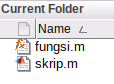
\includegraphics[width=100pt]{images/iconfile}
			\caption{Icon Fungsi dan Skrip}
		\end{figure}
	\end{itemize}

	Untuk membuat file fungsi baru, klik toolbar \textit{HOME} -> \textit{New} -> \textit{Function}.
	Anda akan disuguhkan template bawaan MATLAB untuk fungsi.
	Hapus semua dan ganti dengan contoh fungsi perhitungan tekanan gas ideal berikut.
	Simpan dengan nama file \textbf{presgas.m}.

	\begin{minted}[frame=lines,framesep=2mm,fontsize=\small,bgcolor=LightGray]{matlab}
function p = presgas(n,V,T)
	kB = 1.380649e-23; nA = 6.02214076e+23;
	Tk = T + 273.15;
	p = n*kB*nA*(Tk/V)*9.86923e-6;
end
	\end{minted}

	Misal menghitung tekanan 1 mol gas pada ruang berukuran 2 $m^3$ pada suhu ruang 25\textdegree C melalui Command-Window
	\begin{minted}[frame=lines,framesep=2mm,fontsize=\small,bgcolor=LightGray]{matlab}
>> presgas(1,2,25)
ans =
    0.0122
	\end{minted}

	\subsection{Komentar}

	Komentar adalah statement-statement yang ditambahkan pada kode file sebagai penjelas.
	Komentar tidak dieksekusi oleh MATLAB.

	Beberapa bentuk komentar yang umum digunakan:
	\begin{itemize}
		\item Komentar satu baris dengan diawali tanda persen (\textbf{\%}).
		Umum digunakan untuk penanda atau penjelas suatu baris.

		Contoh:
		\begin{minted}[frame=lines,framesep=2mm,fontsize=\small,bgcolor=LightGray]{matlab}
function p = presgas(n,V,T)
	kB = 1.380649e-23; nA = 6.02214076e+23; % Konstanta gas R
	Tk = T + 273.15;                        % Konversi nilai suhu ke Kelvin
	p = n*kB*nA*(Tk/V)*9.86923e-6;          % Tekanan gas ideal dalam atm
end
		\end{minted}

		\textbf{TIPS:} Anda juga dapat menggunakan komentar untuk "disable" suatu baris statement tanpa harus menghapusnya.
		Anda dapat klik toolbar \textit{Editor} -> \textit{Comment} untuk mempercepat menambahkan tanda komentar pada baris yang dipilih.

		Contoh:
		\begin{minted}[frame=lines,framesep=2mm,fontsize=\small,bgcolor=LightGray]{matlab}
function p = presgas(n,V,T)
	% kB = 1.380649e-23; nA = 6.02214076e+23; % Konstanta gas R
	R = 8.314;

	Tk = T + 273.15;                        % Konversi nilai suhu ke Kelvin

	% p = n*kB*nA*(Tk/V)*9.86923e-6;          % Tekanan gas ideal dalam atm
	p = n*R*(Tk/V)*9.86923e-6;
end
		\end{minted}
		\item Komentar dengan garis pembatas untuk memisahkan topik-topik, diawali tanda persen dobel (\textbf{\%\%}).
		Baik komentar dan garis pembatas tidak mempengaruhi jalannya kode.

		\begin{figure}[!ht]
			\centering
			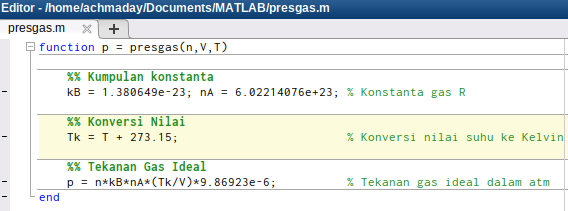
\includegraphics[width=400pt]{images/komentopik}
			\caption{Komentar dengan pembatas topik}
		\end{figure}
	\end{itemize}

	\section{Fungsi Inline/Handler}

	Selain menggunakan file kode fungsi, anda dapat membuat fungsi dengan keyword \textbf{inline} dan operator \textbf{@}.

	\begin{itemize}
		\item \textbf{Inline}. Metode inline dapat digunakan untuk membuat fungsi yang dinyatakan dalam satu baris statement dengan satu input variabel/vektor.
		Entitas fungsi, input, dan output akan diperlakukan oleh MATLAB layaknya entitas objek tersendiri.
		Argumen perintah inline berupa vektor karakter persamaan dan variabel dengan diapit tanpa petik (\textbf{'}).

		Contoh fungsi pangkat 2 untuk variabel x:
		\begin{minted}[frame=lines,framesep=2mm,fontsize=\small,bgcolor=LightGray]{matlab}
>> f = inline('x^2+x+1', 'x');
>> f(5)
ans =
    31
		\end{minted}

		\item \textbf{Handler}. Metode ini digunakan untuk deklarasi fungsi handler menggunakan operator \textbf{@}.
		Pengunaannya mirip dengan metode inline dimana dinyatakan dalam satu baris dan satu input variabel/vektor.
		Operator fungsi @ tidak membutuhkan vektor karakter untuk deklarasi.
		Entitas fungsi, input, dan output akan diperlakukan oleh MATLAB layaknya entitas objek tersendiri.

		\newpage
		Contoh fungsi pangkat 2 untuk variabel x:
		\begin{minted}[frame=lines,framesep=2mm,fontsize=\small,bgcolor=LightGray]{matlab}
>> f = @(x) (x^2+x+1);
>> f(5)
ans =
    31
		\end{minted}

		Fungsi handler akan sangat berguna jika anda ingin suatu file fungsi diperlakukan layaknya entitas objek tersendiri.

		Contoh fungsi gas ideal sebelumnya menggunakan input berupa vektor:
		\begin{minted}[frame=lines,framesep=2mm,fontsize=\small,bgcolor=LightGray]{matlab}
function p = presgas(x)
	n = x(1); V = x(2); T = x(3);

	R = 8.314;
	Tk = T + 273.15;
	p = n*R*(Tk/V)*9.86923e-6;
end
		\end{minted}

		Anda dapat "load" fungsi tersebut sebagai fungsi handler:
		\begin{minted}[frame=lines,framesep=2mm,fontsize=\small,bgcolor=LightGray]{matlab}
>> gas = @(x) (presgas(x));
>> param = [1,2,25];
>> gas(param)
ans =
    0.0122
		\end{minted}
	\end{itemize}

	Jika tidak membutuhkan fungsi sebagai entitas objek/simbolik, maka menggunakan kode file fungsi lebih direkomendasikan (lebih sederhana).

	\newpage
	\section{Kendali Program}

	Kendali program adalah metode untuk mengatur jalannya program, skrip, atau fungsi berdasarkan parameter yang telah ditentukan.
	Kendali yang umum digunakan adalah Percabangan dan Perulangan.

	\subsection{Operator Relational}

	Sebelum melanjutkan, perlu dipahami dahulu operator relational yang dapat digunakan untuk kondisi kendali.
	Operator perbandingan yang umum digunakan.

	\begin{center}
		\begin{tabular}{|c|c|}
			\hline
			Operator & Makna \\
			\hline\hline
			< & Kurang dari \\
			\hline
			<= & Kurang dari atau sama \\
			\hline
			> & Lebih dari \\
			\hline
			>= & Lebih dari atau sama \\
			\hline
			== & sama dengan \\
			\hline
			~= & tidak sama dengan \\
			\hline
			\&\& & logika AND \\
			\hline
			|| & logika OR \\
			\hline
		\end{tabular}
	\end{center}

	\textbf{PERHATIAN:} Bedakan antara simbol \textbf{=} dan \textbf{==}.
	Simbol sama dengan \textbf{=} digunakan untuk assign nilai ke suatu variabel.
	Simbol dobel sama dengan \textbf{==} digunakan untuk cek nilai.\\

	\textbf{PERHATIAN:} Operator \textbf{\&} dan \textbf{|} digunakan untuk operasi logika.
	Sedangkan \textbf{\&\&} dan \textbf{||} untuk cek kondisi logika.
	Namun pada prakteknya, simbol \textbf{\&} dan \textbf{|} juga dapat digunakan untuk cek kondisi logika.

	\subsection{Percabangan IF}

	Percabangan IF adalah metode pemilihan jalannya program berdasarkan suatu kondisi variabel.
	Pola kode:
	\begin{minted}[frame=lines,framesep=2mm,fontsize=\small,bgcolor=LightGray]{matlab}
if(ekspresi)
	statement
end
	\end{minted}

	Contoh membuat fungsi untuk pengecekan bilangan satuan atau bukan.
	Simpan sebagai \textbf{satuan.m}.
	\begin{minted}[frame=lines,framesep=2mm,fontsize=\small,bgcolor=LightGray]{matlab}
function satuan(x)
	if(x < 10)
		disp("bilangan satuan");
	end
end
	\end{minted}

	Tes fungsi tersebut di Command-Window:
	\begin{minted}[frame=lines,framesep=2mm,fontsize=\small,bgcolor=LightGray]{matlab}
>> satuan(3)
bilangan satuan
>> satuan(10)
>>
	\end{minted}

	Selanjutnya jika membutuhkan lebih dari satu kondisi, digunakan keyword \textbf{elseif}.
	Berikut pola kode yang digunakan:
	\begin{minted}[frame=lines,framesep=2mm,fontsize=\small,bgcolor=LightGray]{matlab}
if(ekspresi1)
	statement1
elseif(ekspresi2)
	statement2
end
	\end{minted}

	Contoh berikut fungsi untuk cek nilai satuan dan belasan.
	Simpan dengan nama \textbf{belasan.m}:
	\begin{minted}[frame=lines,framesep=2mm,fontsize=\small,bgcolor=LightGray]{matlab}
function belasan(x)
	if(x>=0 && x<10 )
		disp("bilangan satuan");
	elseif(x>=10 && x<20)
		disp("bilangan belasan");
	end
end
	\end{minted}

	Tes fungsi tersebut di Command-Window:
	\begin{minted}[frame=lines,framesep=2mm,fontsize=\small,bgcolor=LightGray]{matlab}
>> belasan(3)
bilangan satuan
>> belasan(13)
bilangan belasan
>> belasan(30)
>>
	\end{minted}

	Jika membutuh statement yang dapat handle semua kondisi di luar yang disiapkan, digunakan keyword \textbf{else}.
	Pola kode:
	\begin{minted}[frame=lines,framesep=2mm,fontsize=\small,bgcolor=LightGray]{matlab}
if(ekspresi1)
	statement1
elseif(ekspresi2)
	statement2
else
	statement3
end
	\end{minted}

	\textbf{PERHATIAN:} keyword \textbf{else} tidak mendapatkan ekspresi cek kondisi.\\

	Sebagai contoh modifikasi fungsi \textbf{belasan.m} sebelumnya.
	\begin{minted}[frame=lines,framesep=2mm,fontsize=\small,bgcolor=LightGray]{matlab}
function belasan(x)
	if(x>=0 && x<10 )
		disp("bilangan satuan");
	elseif(x>=10 && x<20)
		disp("bilangan belasan");
	else
		disp("diluar rentang");
	end
end
	\end{minted}

	\newpage
	Tes dengan bilangan di luar rentang:
	\begin{minted}[frame=lines,framesep=2mm,fontsize=\small,bgcolor=LightGray]{matlab}
>> belasan(30)
diluar rentang
	\end{minted}

	\subsection{Percabangan SWITCH}

	SWITCH merupakan bentuk lain dari percabangan seperti IF-ELSEIF-ELSE.
	Perbedaannya adalah SWITCH hanya mengevaluasi satu variabel, sedangkan IF mengevaluasi kondisi logika.
	Pola kode:
	\begin{minted}[frame=lines,framesep=2mm,fontsize=\small,bgcolor=LightGray]{matlab}
switch variabel
	case nilai1
		statement1
	case nilai2
		statement2
	otherwise
		statement3
end
	\end{minted}

	Contoh fungsi untuk cek bilangan genap-ganjil.
	Simpan dengan nama \textbf{genap.m}.
	\begin{minted}[frame=lines,framesep=2mm,fontsize=\small,bgcolor=LightGray]{matlab}
function genap(x)
	sisa = mod(x,2);

	switch sisa
		case 0
			disp("Genap");
		case 1
			disp("Ganjil");
		otherwise
			disp("Pecahan");
		end
end
	\end{minted}

	Tes fungsi tersebut:
	\begin{minted}[frame=lines,framesep=2mm,fontsize=\small,bgcolor=LightGray]{matlab}
>> genap(30)
Genap
>> genap(13)
Ganjil
>> genap(0.5)
Pecahan
	\end{minted}

	\newpage
	\subsection{Perulangan WHILE}

	WHILE adalah metode perulangan yang terus berulang selama kondisi ekspresi bernilai benar.
	Pola kode:
	\begin{minted}[frame=lines,framesep=2mm,fontsize=\small,bgcolor=LightGray]{matlab}
initial_ekspresi
while(ekspresi)
	statement
	modifikasi_ekpresi
end
	\end{minted}

	Contoh berikut skrip yang menampilkan kalimat sebanyak 5 kali.
	\begin{minted}[frame=lines,framesep=2mm,fontsize=\small,bgcolor=LightGray]{matlab}
close all;
clear

id = 0;
while(id<5)
	out = "bilangan: " + num2str(id);
	id = id +1;
	disp(out);
end
	\end{minted}

	\textbf{PERHATIAN:} baris '\textbf{id = id + 1;}' adalah \textbf{modifikasi\_expresi} dan sangat penting.
	Jika nilai \textbf{id} tidak berubah dan kondisi \textbf{id<5} selamanya benar, maka loop tidak pernah berhenti dengan sendirinya.\\

	Tes di Command-Window:
	\begin{minted}[frame=lines,framesep=2mm,fontsize=\small,bgcolor=LightGray]{matlab}
>> ulang
bilangan: 0
bilangan: 1
bilangan: 2
bilangan: 3
bilangan: 4
	\end{minted}

	\textbf{TIPS:} Anda juga dapat menuliskan WHILE dalam satu baris jika statement yang diulang sedikit.
	Penulisannya adalah \textbf{while} dan statement pertama dipisah koma, kemudian selebihnya dipisah semi-colon hingga \textbf{end}.
	\begin{minted}[frame=lines,framesep=2mm,fontsize=\small,bgcolor=LightGray]{matlab}
while(ekspresi), statement1; statement2; end;
	\end{minted}

	Contoh perulangan sebelumnya:
	\begin{minted}[frame=lines,framesep=2mm,fontsize=\small,bgcolor=LightGray]{matlab}
>> id = 0
>> while(id<5), disp(id); id = id +1; end;
	\end{minted}

	\subsection{Perulangan FOR}

	FOR juga merupakan perulangan sebagaimana WHILE.
	Perbedaannya adalah perulangan WHILE mengikuti kondisi logika ekspresi,
	sedangkan FOR mengikuti suatu variabel vektor.
	Dengan dipandu oleh suatu vektor, FOR tidak butuh initial\_ekspresi dan modifikasi\_ekspresi.

	\newpage
	Pola kode:
	\begin{minted}[frame=lines,framesep=2mm,fontsize=\small,bgcolor=LightGray]{matlab}
for variabel = deklarasi_vektor
	statement
end
	\end{minted}

	Contoh perulangan sebelumnya ditulis dalam bentuk FOR.
	\begin{minted}[frame=lines,framesep=2mm,fontsize=\small,bgcolor=LightGray]{matlab}
for id = 0:5
	out = "bilangan: " + num2str(id);
	disp(out);
end
	\end{minted}

	Tes di Command-Window:
	\begin{minted}[frame=lines,framesep=2mm,fontsize=\small,bgcolor=LightGray]{matlab}
>> ulang
bilangan: 0
bilangan: 1
bilangan: 2
bilangan: 3
bilangan: 4
bilangan: 5
	\end{minted}

	\textbf{TIPS:} Anda juga dapat menuliskan FOR dalam satu baris jika statement yang diulang sedikit.
	Penulisannya adalah \textbf{for} dan statement pertama dipisah koma, kemudian selebihnya dipisah semi-colon hingga \textbf{end}.
	\begin{minted}[frame=lines,framesep=2mm,fontsize=\small,bgcolor=LightGray]{matlab}
for variabel=deklarasi_vector, statement1; statement2; end;
	\end{minted}

	Contoh perulangan sebelumnya:
	\begin{minted}[frame=lines,framesep=2mm,fontsize=\small,bgcolor=LightGray]{matlab}
>> for id=0:5, disp(id); id = id +1; end;
	\end{minted}

	\section{Plot}

	MATLAB telah menyediakan beragam fungsi built-in untuk plotting.
	Pemilihan fungsi bisa jadi cocok atau juga tidak tergantung vektor/matrix yang akan diplot.

	\subsection{Contoh Plot}

	Berikut beberap contoh fungsi plot:
	\begin{itemize}
		\item \textbf{plot()}. Fungsi ini adalah fungsi dasar plot 2-D axis yang umum digunakan.

		Contoh plot fungsi sin(t) untuk 100 nilai t mulai dari 0 hingga pi.
		\begin{minted}[frame=lines,framesep=2mm,fontsize=\small,bgcolor=LightGray]{matlab}
>> t = 0:pi/100:pi;
>> y = sin(t);
>> plot(t,y);
		\end{minted}

		\newpage
		\begin{figure}[!ht]
			\centering
			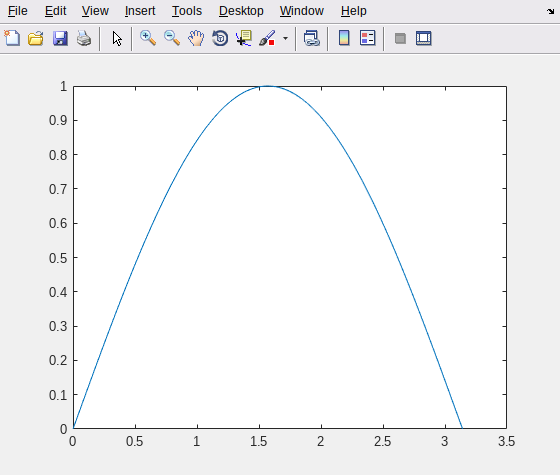
\includegraphics[width=220pt]{images/plot1}
			\caption{Contoh Plot}
		\end{figure}

		Anda juga dapat menggabungkan dua atau lebih plot dalam satu grafik.
		Contoh:
		\begin{minted}[frame=lines,framesep=2mm,fontsize=\small,bgcolor=LightGray]{matlab}
>> t = 0:pi/100:pi;
>> y1 = sin(t);
>> y2 = sin(2*t);
>> plot(t,y1,t,y2);
		\end{minted}

		\begin{figure}[!ht]
			\centering
			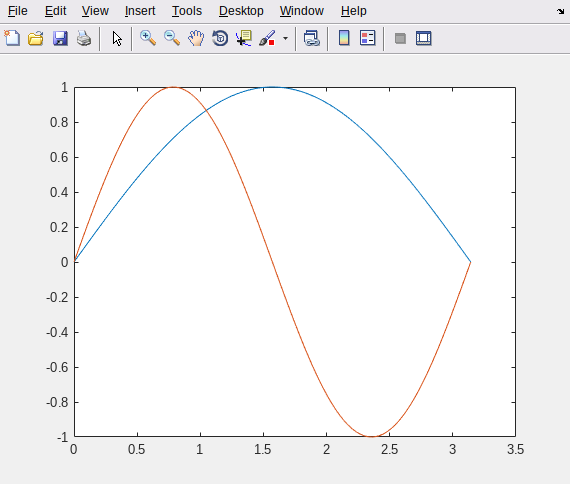
\includegraphics[width=220pt]{images/plot2}
			\caption{Contoh 2 Plot}
		\end{figure}

		\textbf{TIPS:} Anda juga dapat menggabungkan beberapa plot dalam satu grafik dengan perintah \textbf{hold}.

		Contoh:
		\begin{minted}[frame=lines,framesep=2mm,fontsize=\small,bgcolor=LightGray]{matlab}
>> t = 0:pi/100:pi;
>> y1 = sin(t);
>> y2 = sin(2*t);
>> y3 = sin(3*t);
>> plot(t,y1);
>> hold on
>> plot(t,y2);
>> plot(t,y3);
>> hold off
		\end{minted}

		\begin{figure}[!ht]
			\centering
			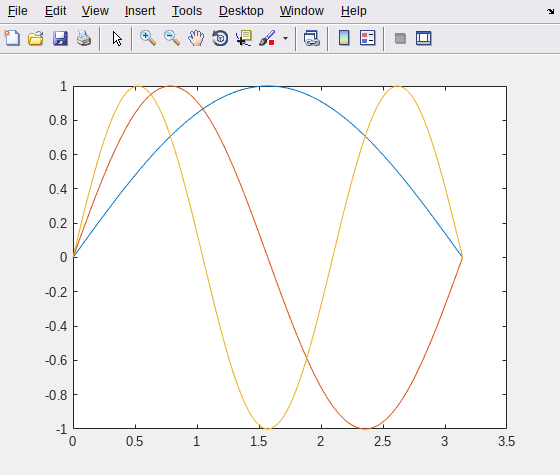
\includegraphics[width=220pt]{images/plot3}
			\caption{Contoh Plot Hold}
		\end{figure}

		\item \textbf{fplot()}. Fungsi ini untuk plotting fungsi simbolik pada rentang nilai input.

		Contoh plot persamaan pangkat 3
		\begin{minted}[frame=lines,framesep=2mm,fontsize=\small,bgcolor=LightGray]{matlab}
>> syms x
>> f = x^3-4*x+3;
>> fplot(f,[-3 3]);
		\end{minted}

		\begin{figure}[!ht]
			\centering
			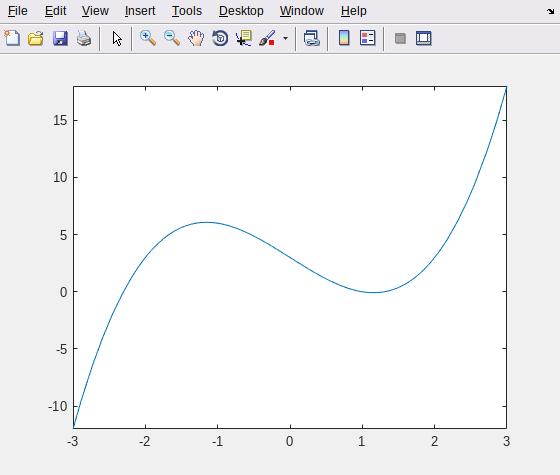
\includegraphics[width=220pt]{images/fplot}
			\caption{Contoh Plot Fungsi simbolik}
		\end{figure}

		\item \textbf{plot3()}. Fungsi ini untuk plotting fungsi dalam 3-D axis.

		Contoh:
		\begin{minted}[frame=lines,framesep=2mm,fontsize=\small,bgcolor=LightGray]{matlab}
>> t = 0:0.1:8*pi;
>> x = 0.8*sin(t);
>> y = 1.2*cos(t);
>> plot3(t,x,y);
>> xlabel('t'), ylabel('x'), zlabel('y');
		\end{minted}

		\newpage
		\begin{figure}[!ht]
			\centering
			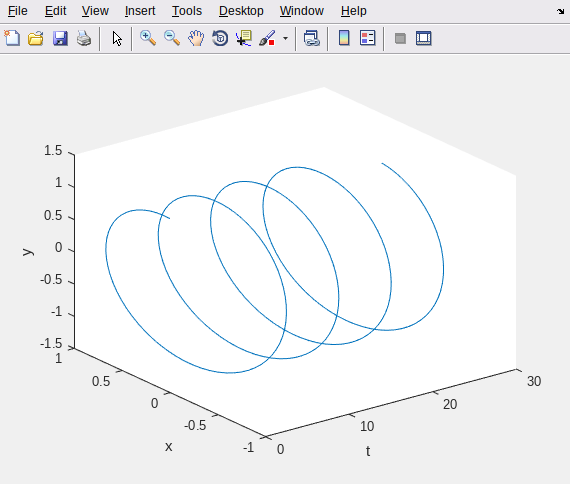
\includegraphics[width=220pt]{images/plot3d}
			\caption{Contoh Plot 3D}
		\end{figure}
	\end{itemize}

	\textbf{TIPS:} Jika membutuhkan jenis plotting lain, silahkan cek help MATLAB di alamat:\\
	\url{https://www.mathworks.com/help/matlab/creating_plots/types-of-matlab-plots.html}

	\subsection{Subplot}

	Subplot adalah menampilkan beberapa plot dalam satu jendela figure baru.
	Subplot akan membuat jendela plot baru dan menaruh plot sesuai urutan.
	Pola perintahnya:
	\begin{minted}[frame=lines,framesep=2mm,fontsize=\small,bgcolor=LightGray]{matlab}
figure()
subplot(jumlah_baris, jumlah_kolom, posisi_urutan);
fungsi_plot();
	\end{minted}

	Contoh menampilkan grafik plot sinus dalam 2x2 subplot dalam sebuah skrip:
	\begin{minted}[frame=lines,framesep=2mm,fontsize=\small,bgcolor=LightGray]{matlab}
close all;
clear;

t = 0:pi/100:pi;

figure();

y1 = sin(2*t);
subplot(2,2,1);
plot(t,y1);

y2 = sin(4*t);
subplot(2,2,2);
plot(t,y2);

y3 = sin(8*t);
subplot(2,2,3);
plot(t,y3);

y4 = sin(16*t);
subplot(2,2,4);
plot(t,y4);
	\end{minted}

	Jika diperhatikan, setiap subplot hanya berbeda index, namun jumlah baris dan kolom posisi plot tetap sama (2x2).

	\begin{figure}[!ht]
		\centering
		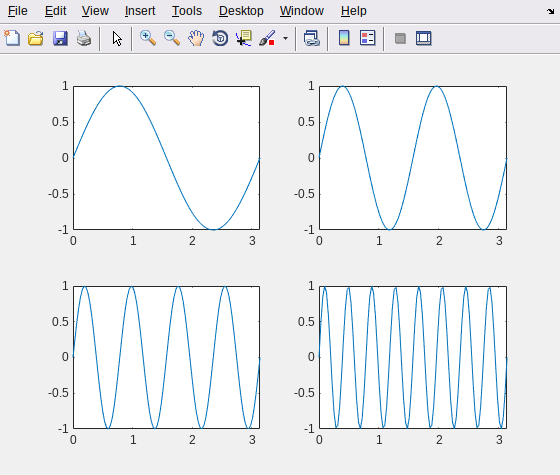
\includegraphics[width=300pt]{images/subplot}
		\caption{Contoh Subplot}
	\end{figure}

	\section{File Input/Output}

	Matlab mendukung proses pembacaan dan penulisan variable ke dalam suatu berkas.
	Disini akan dibahas dua format berkas, yaitu MAT-File \textbf{*.mat} dan teks CSV \textbf{*.csv}.

	\subsection{MAT}

	Format berkas MAT adalah format binary (bukan teks) yang dapat menyimpan seluruh konten workspace.
	Fungsi yang digunakan adalah \textbf{save()}.
	Berikut contohnya:

	\begin{minted}[frame=lines,framesep=2mm,fontsize=\small,bgcolor=LightGray]{matlab}
var1 = linspace(0,10,10);
save('coba.mat');
	\end{minted}

	\begin{figure}[!ht]
		\centering
		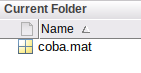
\includegraphics[width=150pt]{images/matfile}
		\caption{Contoh MAT-File}
	\end{figure}

	Kita dapat pula menyimpan variabel spesifik (tidak seluruh workspace) dengan menambahkan argumen nama variabel,
	contohnya:

	\begin{minted}[frame=lines,framesep=2mm,fontsize=\small,bgcolor=LightGray]{matlab}
var1 = linspace(0,10,10);
save('coba.mat','var1');
	\end{minted}

	Selanjutnya untuk memasukkan berkas MAT, dapat menggunakan fungsi \textbf{load()}.
	Berikut contohnya:
	\begin{minted}[frame=lines,framesep=2mm,fontsize=\small,bgcolor=LightGray]{matlab}
clear all
load('coba.mat');
	\end{minted}

	\textbf{TIPS:} Selain menggunakan kedua fungsi di atas, dapat pula digunakan context menu \textbf{Save As} pada panel Workspace
	dan \textbf{Import} pada panel Current Folder.

	\subsection{CSV}

	Format berkas CSV atau Comma Separated Value adalah format teks (non-binary) bersifat terbuka yang kompatibel dengan banyak program lain.
	Fungsi yang dapat digunakan adalah \textbf{csvwrite()}.
	Berikut contoh menulis CSV pada suatu matrix hasil sinus:
	\begin{minted}[frame=lines,framesep=2mm,fontsize=\small,bgcolor=LightGray]{matlab}
x = linspace(0,1,10);
y = sin(x);
z = [x;y];
csvwrite('tes.csv',z');
	\end{minted}

	\begin{figure}[!ht]
		\centering
		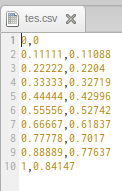
\includegraphics[width=150pt]{images/csvfile}
		\caption{Contoh isi CSV File}
	\end{figure}

	Untuk membaca berkas CSV, dapat digunakan fungsi \textbf{csvread()}.
	Perlu diperhatikan bahwa fungsi ini memiliki tiga syarat:
	\begin{enumerate}
		\item Berkas CSV hanya berisi numerik dan tidak ada alphabet
		\item Kolom data tidak memiliki header
		\item Delimiter benar-benar karakter koma
	\end{enumerate}
	Contoh:
	\begin{minted}[frame=lines,framesep=2mm,fontsize=\small,bgcolor=LightGray]{matlab}
clear all
z = csvread('tes.csv');
	\end{minted}

	\newpage
	\section{Penugasan}

	Buat file fungsi/skrip plotting logo MATLAB.
	Plot logo MATLAB dalam 4 subplot dengan masing-masing berbeda warna dasar.
	Submit file fungsi/skrip tersebut.
	Beri komentar tiap barisnya sebagai penjelasan.\\

	\textbf{TIPS:} Anda dapat melihat webpage berikut sebagai referensi:\\
	\url{https://www.mathworks.com/help/matlab/visualize/creating-the-matlab-logo.html}

	\newpage
	\chapter{Pemrograman Lanjut}

	Pada Bab Pemrograman Lanjut lebih diarahkan kepada penggunaan MatLab secara implementatif.
	Untuk bagian materi ini, diasumsikan bahwa pembaca telah cukup familiar dengan Matlab baik antar muka program dan bahasanya.

	\section{Koneksi Hardware}

	Dalam dunia elektronika industri, tersedia beragam protokol komunikasi data yang dapat digunakan untuk pertukaran data baik numerik atau teks.
	Antara lain seperti:
	\begin{enumerate}
		\item I2C (Inter IC Connection)
		\item USART (Universal Synchronous/Asynchronous Receiver Transmitter)
		\item USB (Universal Serial Bus)
		\item SPI (Serial Peripheral Interface)
		\item CAN (Controlled Area Network)
		\item TCP/IP melalui WiFi atau Ethernet
	\end{enumerate}

	\textbf{PERHATIAN:} Untuk kebutuhan komunikasi dengan hardware, tidak disarankan menggunakan Matlab Online
	karena webrowser tidak dapat mengakses driver serial port.

	Disini Matlab menyediakan dukungan untuk komunikasi data text dengan protokol serial USART yang dikonversi ke USB.

	Beberapa produk yang dapat digunakan sebagai USART/USB konverter, atau telah terintegrasi pada board:
	\begin{itemize}
		\item Board Arduino seri Uno, Nano, dan Mega
		\item Board NodeMCU ESP32 dan ESP8266
		\item Board STM32 Discovery, Nucleo, dan BluePill menyediakan port untuk USB-CDC
		\item Konverter TTL-USB berbasis chip CH340x, FT232RL, atau PL2303
	\end{itemize}

	Untuk contoh disini, digunakan NodeMCU ESP32 yang terhubung ke laptop melalui USB.

	\begin{figure}[!ht]
		\centering
		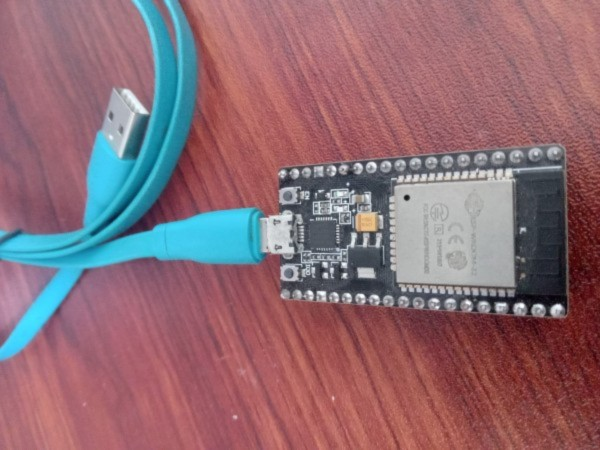
\includegraphics[width=150pt]{images/esp32nodemcu}
		\caption{Contoh NodeMCU ESP32}
	\end{figure}

	Untuk kebutuhan demo simulasi disini, unit NodeMCU akan diprogram untuk mengirim data dummy setiap mendapat perintah \textbf{data}.

	\newpage
	\subsection{Install ESP32-Arduino}
	Sebelum dapat menyambung koneksi laptop, jika menggunakan OS Windows, maka terlebih dahulu install driver untuk chip CP2102.
	Driver dapat diunduh di halaman:\\
	\url{https://www.silabs.com/developers/usb-to-uart-bridge-vcp-drivers?tab=downloads}\\

	Kemudian, install Arduino IDE versi 1.8.16 dari halaman berikut:\\
	\url{https://www.arduino.cc/en/software/OldSoftwareReleases}\\

	Selanjutnya, install ESP32 Framework dengan mengikuti tutorial berikut:\\
	\url{https://github.com/mekatronik-achmadi/md_tutorial/blob/master/electronic/tutorials/esp32_arduino.md}

	\subsection{Sourcecode ESP32}

	Berikut kode sumber yang dapat diupload ke Unit NodeMCU ESP32 dengan Arduino IDE:

	\begin{minted}[frame=lines,framesep=2mm,fontsize=\small,bgcolor=LightGray]{c}
#define LED_BUILTIN GPIO_NUM_2

void toggleLED(void * parameter){
	while(1){
		digitalWrite(LED_BUILTIN, HIGH); vTaskDelay(500 / portTICK_PERIOD_MS);
		digitalWrite(LED_BUILTIN, LOW); vTaskDelay(500 / portTICK_PERIOD_MS);
	}
}

void setup() {
	Serial.begin(9600);
	pinMode(LED_BUILTIN, OUTPUT);
	xTaskCreate(toggleLED,"Toggle LED",1000,NULL,10,NULL);
}

void loop() {
	if(Serial.available()){
		String cmd = Serial.readStringUntil('\r');
		if(cmd=="data"){
			Serial.println(random(20));
		}
		else{
			Serial.println("Command Error:");
		}
	}
}
	\end{minted}

	Secara umum, kode sumber ESP32 menjalankan dua hal secara simultan:
	\begin{enumerate}
		\item Membuat LED berkedip
		\item Mengirimkan angka sembarang melalui jalur Serial UART
	\end{enumerate}

	\subsection{Sourcecode Matlab}

	\textbf{PERHATIAN:} Untuk sistem operasi GNU/Linux dan juga mungkin MacOS,
	perlu dilakukan modifikasi akses terhadap file descriptor dari serial port.
	Contoh perintah di shell anda:

	\begin{minted}[frame=lines,framesep=2mm,fontsize=\small,bgcolor=LightGray]{bash}
sudo chmod +777 /run/lock
sudo chmod +777 /dev/ttyUSB0
	\end{minted}

	Berikut kode sumber di Matlab untuk melakukan "request" sejumlah 10 angka sembarang NodeMCU ESP32.

	\begin{minted}[frame=lines,framesep=2mm,fontsize=\small,bgcolor=LightGray]{matlab}
clear;
clc;

% instrreset
% instrhwinfo('serial')

devport = serial('/dev/ttyUSB0',...
'BaudRate',9600,...
'DataBits',8,...
'Parity','none',...
'StopBits',1,...
'Terminator','CR'); % atau CR/LF sesuai program di chip

% instrfind
% devport.InputBufferSize = 1000000;

fopen(devport);

data = 0;
i = 1;
while(i<11)
	fprintf(devport,'data');
	recv = str2double(fscanf(devport));
	if(isnan(recv))
		disp('value NaN');
	else
		disp("angka: " + num2str(recv));
		data(i) = recv;
		i = i +1;
	end
	pause(1);
end

fclose(devport);
delete(devport);

disp(data);
	\end{minted}

	\newpage
	\section{Solving ODE}

	menyusul

	\section{Numerical Method}

	menyusul

	\section{Spesific Implementation}

	menyusul

	\chapter{Bonus: Git-SCM}

	Git SCM (Source Code Manager) adalah program untuk merekam dan tracking isi file (terutama file teks).
	Selain itu Git digunakan untuk mengolah modifikasi kode (patch) sehingga bisa diterapkan
	model pengembangan program yang bersifat kolaboratif.\\

	\textbf{PERHATIAN:} Bagian ini bukan merupakan pembahasan MATLAB.
	Namun tool tambahan untuk mempermudah proses pengembangan program.

	\section{Git-CLI}

	Berikut akan dibahas program Git CLI.
	Program ini adalah program utama Git yang berjalan di CLI (Command-Line Interface).

	\subsection{Instalasi}

	Berikut instalasi paket program Git:
	\begin{itemize}
		\item \textbf{Windows}. Download installer Windows Setup (jangan yang portable) disini:\\
		\url{https://git-scm.com/download/win}

		\item \textbf{ArchLinux/Manjaro}. Berikut perintah instalasi untuk distro ArchLinux/Manjaro dan turunannya:
		\begin{minted}[frame=lines,framesep=2mm,fontsize=\small,bgcolor=LightGray]{sh}
$> sudo pacman -S git tig
		\end{minted}
	\end{itemize}

	Selanjutnya buat folder baru kosong (contoh disini dinamai \textbf{git-coba}).
	Masuk ke folder tersebut, kemudian klik-kanan ruang kosong dalam folder tersebut.
	Kemudian pilih \textit{Git Bash Here}.

	\begin{figure}[!ht]
		\centering
		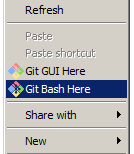
\includegraphics[width=100pt]{images/githere0}
		\caption{Konteks Menu Git Bash}
	\end{figure}

	\newpage
	Kemudian akan muncul jendela Git-CLI.
	Coba masukkan perintah berikut (tanda \textbf{\$} sebagai Prompt):
	\begin{minted}[frame=lines,framesep=2mm,fontsize=\small,bgcolor=LightGray]{sh}
$ git --version
	\end{minted}

	\begin{figure}[!ht]
		\centering
		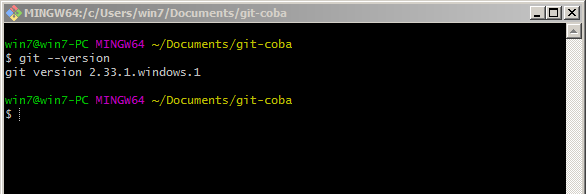
\includegraphics[width=400pt]{images/git0}
		\caption{Versi Git Terinstall}
	\end{figure}

	\subsection{Mendaftarkan ID}

	Sebelum melanjutkan, masukkan nama dan email agar Git bisa mencantumkan ID saat modifikasi kode.
	Contoh ID nama dan email penulis.
	\begin{minted}[frame=lines,framesep=2mm,fontsize=\small,bgcolor=LightGray]{sh}
$ git config --global user.name "Achmadi"
$ git config --global user.email "mekatronik.achmadi@gmail.com"
	\end{minted}

	\subsection{Git Repository}

	Selanjutnya untuk membuat repository Git baru, masukkan perintah CLI berikut di alamat folder \textbf{git-coba} tadi.
	\begin{minted}[frame=lines,framesep=2mm,fontsize=\small,bgcolor=LightGray]{sh}
$ git init
	\end{minted}

	\begin{figure}[!ht]
		\centering
		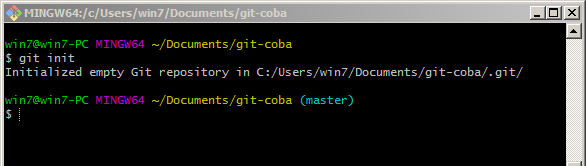
\includegraphics[width=400pt]{images/git1}
		\caption{Inisiasi Repo Git}
	\end{figure}

	Terlihat pada prompt CLI sekarang ditambahkan nama branch (master).
	Penjelasan term Branch dan cara Branching akan dibahas di bagian selanjutnya.

	\newpage
	Selain prompt yang berubah, juga akan muncul folder hidden \textbf{.git}.
	Jangan modifikasi isi folder ini kecuali melalui program Git.

	\begin{figure}[!ht]
		\centering
		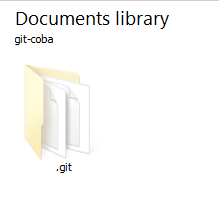
\includegraphics[width=150pt]{images/git2}
		\caption{Folder-Sistem Git}
	\end{figure}

	\subsection{Menambahkan File untuk Tracking}

	Berikut contoh workflow untuk manajemen versi kode sumber.
	Buat skrip baru seperti berikut:
	\begin{minted}[frame=lines,framesep=2mm,fontsize=\small,bgcolor=LightGray]{matlab}
close all;
clear;

syms x y;

z = x^3 - 3*x^2*y + 3*x*y^2 - y^3;
z1 = diff(z,x);
z2 = diff(z,x,2);
	\end{minted}

	Simpan dengan nama \textbf{coba.m} dalam folder \textbf{git-coba} (jangan di dalam folder \textbf{.git}).

	Saat ada file baru, program Git tidak otomatis merekam dan tracking isi file tersebut.
	Perlu ditambahkan sebagai file tracked.

	Pertama, cek status repo dengan perintah:
	\begin{minted}[frame=lines,framesep=2mm,fontsize=\small,bgcolor=LightGray]{sh}
$ git status
	\end{minted}

	Akan tampil bahwa file \textbf{coba.m} sebagai file baru unstaged (merah).

	\begin{figure}[!ht]
		\centering
		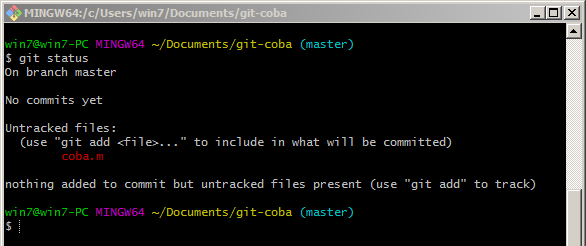
\includegraphics[width=400pt]{images/git3}
		\caption{File Baru}
	\end{figure}

	Kemudian tambahkan file tersebut ke \textbf{staged}.
	Status staged maksudnya adalah status dimana file dipilih untuk direkam.
	Perintah:
	\begin{minted}[frame=lines,framesep=2mm,fontsize=\small,bgcolor=LightGray]{sh}
$ git add coba.m
	\end{minted}

	\textbf{TIPS:} Jika file yang akan ditambahkan ke staged lebih dari,
	dapat juga digunakan simbol wildcard (\textbf{*}) untuk menambahkan semua.
	\begin{minted}[frame=lines,framesep=2mm,fontsize=\small,bgcolor=LightGray]{sh}
$ git add *
	\end{minted}

	Cek kembali dengan \textbf{git status}, maka akan dikenali sebagai file baru staged (hijau):

	\begin{figure}[!ht]
		\centering
		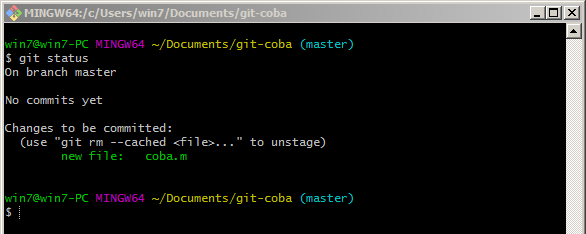
\includegraphics[width=400pt]{images/git4}
		\caption{File Baru Staged}
	\end{figure}

	Selanjutnya untuk membekukan rekaman isi file, tambahkan ke status Commit.
	Status Commit maksudnya adalah status dimana isi file telah untuk direkam.
	Perintah:
	\begin{minted}[frame=lines,framesep=2mm,fontsize=\small,bgcolor=LightGray]{sh}
$ git commit -m "file skrip baru"
	\end{minted}

	\textbf{PERHATIAN:} Opsi \textbf{-m} atau message adalah untuk label pesan commit.
	Usahakan pesan commit singkat dan cukup deskriptif.

	\begin{figure}[!ht]
		\centering
		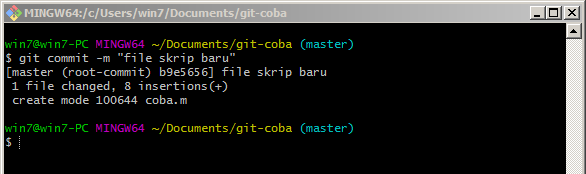
\includegraphics[width=400pt]{images/git5}
		\caption{File Baru Commit}
	\end{figure}

	Disitu terlihat rangkuman berapa banyak file yang berubah dan banyak baris yang ditambahkan.

	\newpage
	Selanjutnya jika anda cek \textbf{git status}, maka folder git dinyatakan bersih dari modifikasi yang tidak terekam.

	\begin{figure}[!ht]
		\centering
		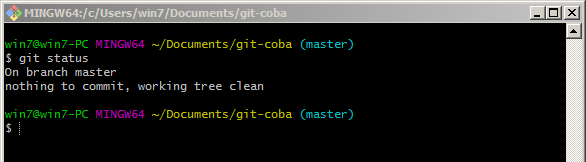
\includegraphics[width=400pt]{images/git6}
		\caption{Folder Git Bersih}
	\end{figure}

	\subsection{Menambahkan Modifikasi File}

	Selanjutnya dicoba melakukan modifikasi pada file \textbf{coba.m}.
	Tambahkan baris berikut di akhir file:
	\begin{minted}[frame=lines,framesep=2mm,fontsize=\small,bgcolor=LightGray]{matlab}
sz = subs(z,[x,y],[2,5]);
sz1 = subs(z1,[x,y],[2,5]);
sz2 = subs(z2,[x,y],[2,5]);
	\end{minted}

	Jika cek \textbf{git status}, maka file akan kembali menjadi unstaged (merah).
	Kemudian sekarang ada label tambahan \textbf{modified}.

	\begin{figure}[!ht]
		\centering
		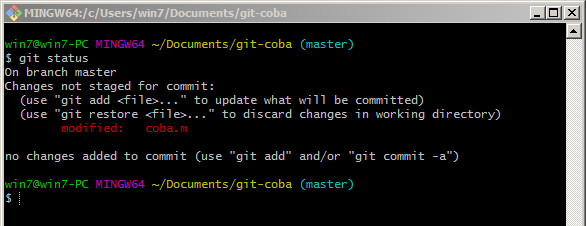
\includegraphics[width=400pt]{images/git7}
		\caption{File Modified}
	\end{figure}

	Sama seperti sebelum, tambahkan file termodifikasi ke status staged:
	\begin{minted}[frame=lines,framesep=2mm,fontsize=\small,bgcolor=LightGray]{sh}
$ git add coba.m
	\end{minted}

	\textbf{TIPS:} Anda dapat gunakan tombol panah atas (\keys{$\uparrow$}) untuk mencari history perintah seperti Command-Window pada MATLAB.
	Anda tinggal pilih dengan tombol panah atas (\keys{$\uparrow$}) dan panah bawah (\keys{$\downarrow$}).
	Tekan ENTER (\keys{\return}) untuk mengeksekusi perintah yang dipilih.

	\newpage
	Cek kembali dengan \textbf{git status}, maka akan dikenali sebagai file modified staged (hijau):
	\begin{figure}[!ht]
		\centering
		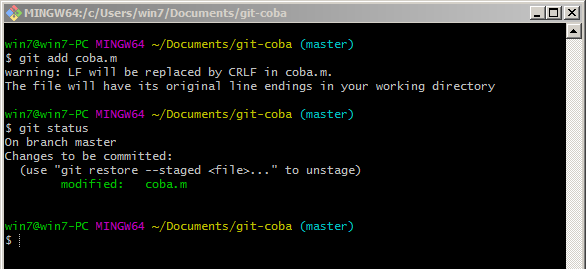
\includegraphics[width=400pt]{images/git8}
		\caption{File Modified Staged}
	\end{figure}

	Sama seperti sebelumnya, lakukan Commit untuk membekukan rekam modifikasi.
	Usahakan pesan commit berbeda dengan sebelumnya.
	\begin{minted}[frame=lines,framesep=2mm,fontsize=\small,bgcolor=LightGray]{sh}
$ git commit -m "tambah substitusi"
	\end{minted}

	\begin{figure}[!ht]
		\centering
		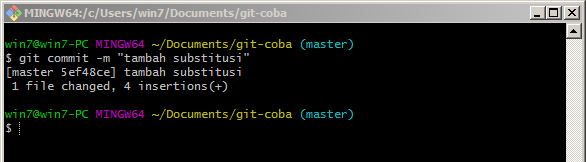
\includegraphics[width=400pt]{images/git9}
		\caption{File Modified Commit}
	\end{figure}

	Terlihat summary commit dengan 1 file berubah dan 4 baris baru ditambahkan.

	\subsection{Modifikasi Sekali Lagi}

	Lakukan modifikasi sekali lagi dengan menambahkan baris berikut ke skrip \textbf{coba.m}:
	\begin{minted}[frame=lines,framesep=2mm,fontsize=\small,bgcolor=LightGray]{matlab}
out = "nilai sz: " + string(sz) +...
",sz1: " + string(sz1) +...
",sz2: " + string(sz2);

disp(out);
	\end{minted}

	Kemudian untuk Commit Modifikasi, perintah berurutan:
	\begin{minted}[frame=lines,framesep=2mm,fontsize=\small,bgcolor=LightGray]{sh}
$ git add coba.m
$ git commit -m "tambah nilai out"
	\end{minted}

	\newpage
	\subsection{Melihat History}

	Selanjutnya untuk melihat history modifikasi gunakan perintah:
	\begin{minted}[frame=lines,framesep=2mm,fontsize=\small,bgcolor=LightGray]{sh}
$ tig
	\end{minted}

	Terlihat history modifikasi.
	Gunakan keyboard panah atas (\keys{$\uparrow$}) dan panah bawah (\keys{$\downarrow$}) untuk memilih commit
	Tekan ENTER (\keys{\return}) untuk melihat isi modifikasi.
	Untuk navigasi di tampilan modifikasi file, gunakan huruf \keys{j} untuk ke bawah dan \keys{k} untuk ke atas.

	\begin{figure}[!ht]
		\centering
		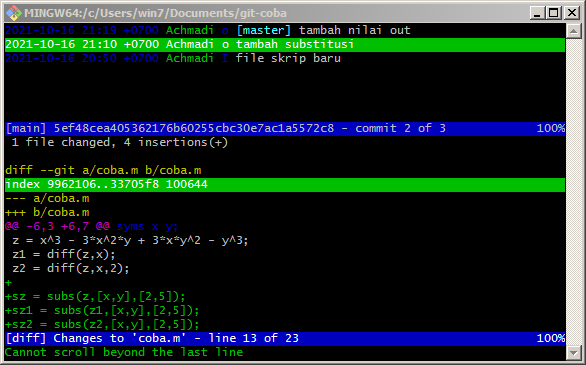
\includegraphics[width=400pt]{images/git10}
		\caption{History Commit}
	\end{figure}

	Cara membaca file modifikasi (patch):
	\begin{itemize}
		\item Cari baris berwarna ungu dan berisi simbol \textbf{@@} dan angka-angka.
		Angka-angka trsebut menunjukkan baris dan kolom dari file aktual

		\item Baris warna putih dibawah baris simbol \textbf{@@} adalah baris modifikasi sebelumnya dan tidak dimodifikasi.

		\item Baris warna hijau dibawah baris simbol \textbf{@@} adalah baris baru yang ditambahkan pada modifikasi ini.

		\item Baris warna merah dibawah baris simbol \textbf{@@} adalah baris lama yang dihapus pada modifikasi ini.
	\end{itemize}

	Untuk keluar dari program \textbf{tig}, gunakan kombinasi tombol CTRL+c (menekan tombol \keys{Ctrl} dan huruf \keys{c} bersamaan di keyboard).

	Diharapkan dengan menggunakan Git-SCM, tidak perlu lagi ada skrip bernama \textbf{coba\_0.m}, \textbf{coba\_bismillah.m}, \textbf{coba\_tolong.m}, dst
	untuk menyimpan beberapa modifikasi dari file yang sama.
	Semua cukup menggunakan tracking Git-SCM untuk menyimpan history modifikasi (patch).

	\begin{figure}[!ht]
		\centering
		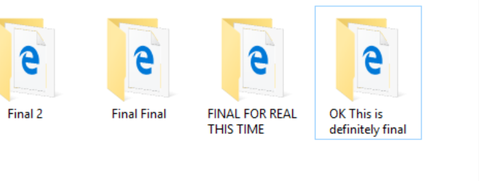
\includegraphics[width=210pt]{images/memescm}
		\caption{contoh SCM yang tidak efektif}
	\end{figure}

	\newpage
	\section{Git-GUI}

	Git-GUI adalah program antar muka GUI yang ditulis dengan widget Tkinter.
	Git-GUI menyediakan paradigma perintah klik icon dan graphical display untuk Git-CLI.\\

	\textbf{PERHATIAN:} Pelajari Git-CLI lebih dahulu untuk memahami konsep workflow Git-SCM.\\

	Untuk akses Git-GUI, klik-kanan ruang kosong dalam suatu folder.
	Kemudian pilih \textit{Git GUI Here}.

	\begin{figure}[!ht]
		\centering
		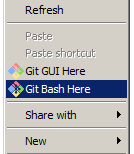
\includegraphics[width=80pt]{images/githere0}
		\caption{Konteks Menu Git GUI}
	\end{figure}

	Tampilan jendela awal akan bergantung apakah pada folder terdapat folder \textbf{.git} atau tidak.

	\begin{figure}[!ht]
		\centering
		\begin{subfigure}[b]{0.25\textwidth}
			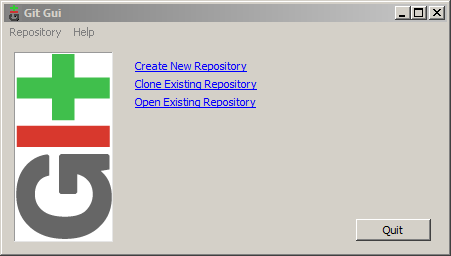
\includegraphics[width=\textwidth]{images/gitgui0}
			\caption{Folder tanpa Git}
		\end{subfigure}
		\begin{subfigure}[b]{0.55\textwidth}
			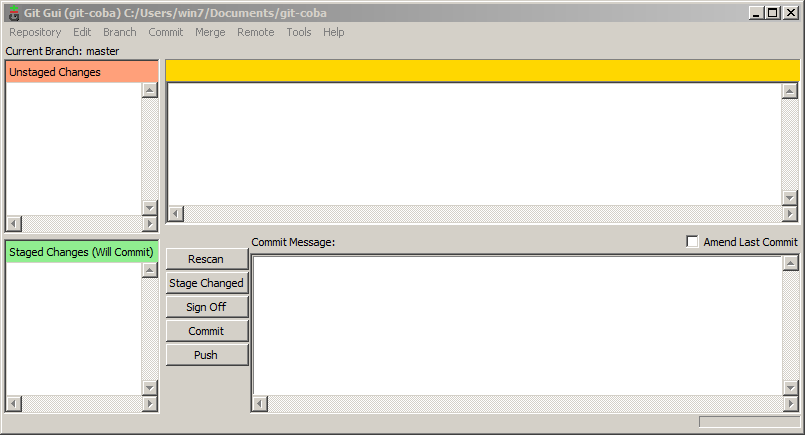
\includegraphics[width=\textwidth]{images/gitgui1}
			\caption{Folder dengan Git}
		\end{subfigure}
		\caption{Jendela awal Git-GUI}
	\end{figure}

	Git GUI juga menyediakan jendela Git History.

	\begin{figure}[!ht]
		\centering
		\begin{subfigure}[b]{0.45\textwidth}
			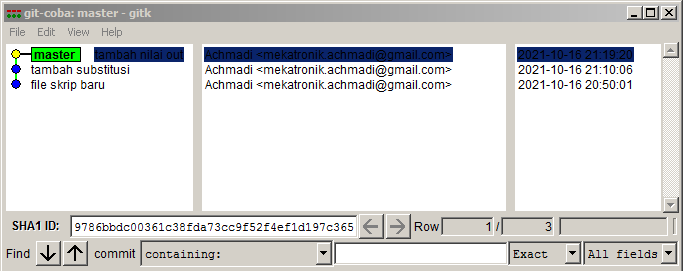
\includegraphics[width=\textwidth]{images/gitgui2}
			\caption{History Commit}
		\end{subfigure}
		\begin{subfigure}[b]{0.45\textwidth}
			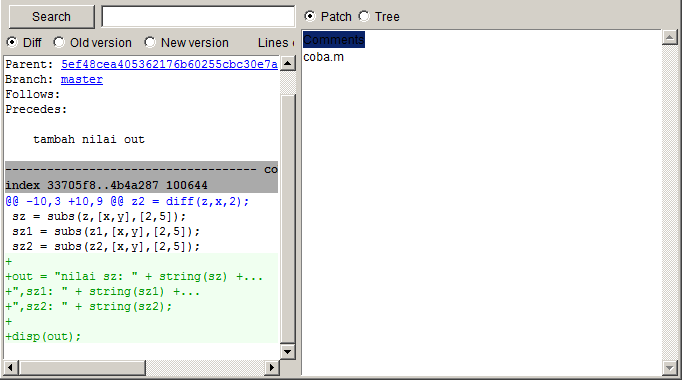
\includegraphics[width=\textwidth]{images/gitgui3}
			\caption{Patch}
		\end{subfigure}
		\caption{Git History}
	\end{figure}

	Penjelasan detil Git-GUI akan dibahas di kesempatan selanjutnya.

	\newpage
	\section{GitHub}

	GitHub adalah situs asuhan Microsoft yang menyimpan Git-Repository baik secara gratis maupun berbayar.
	Dengan GitHub, anda dapat membuat remote repository yang dapat saling tracking dengan local Git repository.
	Selain sebagai back-up, GitHub juga dapat digunakan sebagai pusat pengembangan suatu kode sumber via internet.

	\begin{figure}[!ht]
		\centering
		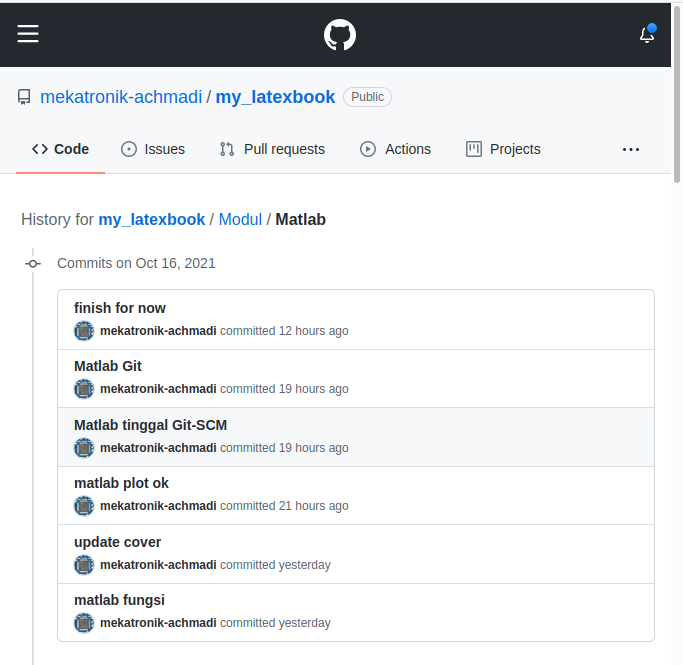
\includegraphics[width=400pt]{images/github0}
		\caption{Contoh Commit History di GitHub}
	\end{figure}

	Penjelasan detil GitHub akan dibahas di kesempatan selanjutnya.

\end{document}